\documentclass[12pt,a4paper]{report}

\usepackage[T1]{fontenc}
\IfFileExists{newtxtext.sty}{\usepackage{newtxtext,newtxmath}}{\usepackage{mathptmx}}
\usepackage{microtype}
\usepackage[a4paper,left=25mm,right=25mm,top=25mm,bottom=25mm]{geometry}
\usepackage{amsmath,amssymb,bm}
\usepackage{graphicx,float,booktabs,array,tabularx,longtable,multirow}
\usepackage[table]{xcolor}
\usepackage{caption}
\captionsetup{font=small,labelfont=bf}
\usepackage{enumitem}
\setlist{itemsep=2pt,topsep=4pt}
\usepackage{tikz}
\usetikzlibrary{arrows.meta,positioning,calc,decorations.pathreplacing,shapes.geometric}
\usepackage{pgfplots}
\pgfplotsset{compat=1.17}
\usepackage[most]{tcolorbox}
\usepackage[colorlinks=true,citecolor=blue,urlcolor=blue,linkcolor=blue]{hyperref}

\setlength{\parindent}{0pt}
\setlength{\parskip}{6pt}
\renewcommand{\arraystretch}{1.2}

% ----- chapters show only "N. Title", as in the previous report
\usepackage{titlesec}
\titleformat{\chapter}{\normalfont\huge\bfseries}{\thechapter.}{0.5em}{}
\titlespacing*{\chapter}{0pt}{0pt}{10pt}

% ----- header / footer
\usepackage{fancyhdr}
\pagestyle{fancy}
\fancyhf{}
\lhead{Study guide: Heat at the Tail}
\rhead{\thepage}
\renewcommand{\headrulewidth}{0.4pt}
\fancypagestyle{plain}{\fancyhf{}\lhead{Study guide: Heat at the Tail}\rhead{\thepage}\renewcommand{\headrulewidth}{0.4pt}}

% ----- boxes
\newtcolorbox{keyidea}[1][]{colback=blue!4,colframe=blue!55!black,boxrule=0.6pt,arc=2pt,left=6pt,right=6pt,top=4pt,bottom=4pt,fonttitle=\bfseries\small,title={#1}}
\newtcolorbox{example}[1][]{colback=orange!6,colframe=orange!70!black,boxrule=0.6pt,arc=2pt,left=6pt,right=6pt,top=4pt,bottom=4pt,fonttitle=\bfseries\small,title={#1}}
\newtcolorbox{sayit}{colback=green!5,colframe=green!45!black,boxrule=0.6pt,arc=2pt,left=6pt,right=6pt,top=4pt,bottom=4pt,fonttitle=\bfseries\small,title={How to say it in the presentation}}

% ----- tikz styles shared by all figures
\tikzset{
  bx/.style={draw=black!55,rounded corners=2pt,align=center,font=\footnotesize,inner sep=4pt,minimum height=1.0cm},
  bdat/.style={bx,fill=black!4},
  blue box/.style={bx,fill=blue!8,draw=blue!55!black},
  orange box/.style={bx,fill=orange!12,draw=orange!70!black},
  green box/.style={bx,fill=green!8,draw=green!45!black},
  red box/.style={bx,fill=red!8,draw=red!60!black},
  ar/.style={-{Stealth[length=2.2mm]},thick,draw=black!65}}

\begin{document}

% =========================================================================
% TITLE PAGE
% =========================================================================
\thispagestyle{empty}
\begin{center}
{\large\em Study guide for the Major Technical Project}\\[4ex]
{\LARGE\bf Heat at the Tail}\\[2ex]
{\Large Understanding every term and step of\\ ``Extreme Value-Guided Deep Generative Models for Imbalanced Classification''}\\[5ex]
{\large\bf Divyansh Jain}\\[1ex]
{\large B23397}\\[1ex]
{\large School of Mathematical and Statistical Sciences, IIT Mandi}\\[1ex]
{\large Supervisor: Dr. Rishikesh Yadav}\\[6ex]
\end{center}

\begin{keyidea}[What this guide is]
This is a personal learning document, not the project report. It explains, in plain words and with pictures, every
idea, term and number used in the project, in the order you need them: the data, what an extreme day is, how the data
are turned into rows, why rare classes are hard, extreme value theory, the three generative models, the classifier, how
results are measured, and what was found. Each chapter ends with a short ``how to say it'' box, and the last pages hold
likely questions and a glossary. All numbers are the project's own results, checked against the code and the result
files.
\end{keyidea}

\vfill
\begin{center}
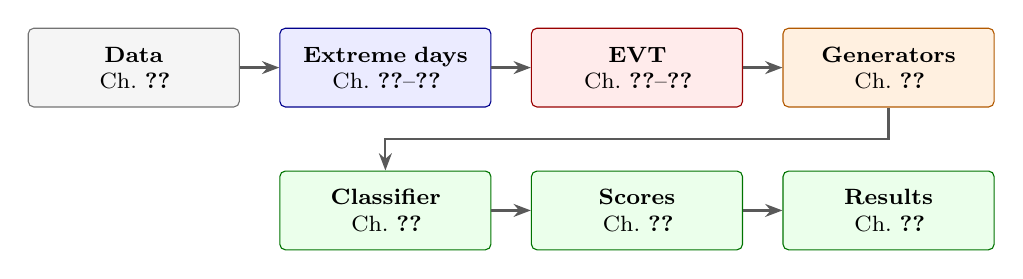
\begin{tikzpicture}[node distance=5mm]
\node[bdat,text width=2.4cm] (a) {\textbf{Data}\\Ch.~\ref{ch:data}};
\node[blue box,text width=2.4cm,right=of a] (b) {\textbf{Extreme days}\\Ch.~\ref{ch:extreme}--\ref{ch:rows}};
\node[red box,text width=2.4cm,right=of b] (c) {\textbf{EVT}\\Ch.~\ref{ch:imb}--\ref{ch:evt}};
\node[orange box,text width=2.4cm,right=of c] (d) {\textbf{Generators}\\Ch.~\ref{ch:gen}};
\node[green box,text width=2.4cm,below=8mm of b] (e) {\textbf{Classifier}\\Ch.~\ref{ch:clf}};
\node[green box,text width=2.4cm,right=of e] (f) {\textbf{Scores}\\Ch.~\ref{ch:metrics}};
\node[green box,text width=2.4cm,right=of f] (g) {\textbf{Results}\\Ch.~\ref{ch:results}};
\draw[ar] (a) -- (b); \draw[ar] (b) -- (c); \draw[ar] (c) -- (d);
\draw[ar] (d.south) |- ++(0,-0.4) -| (e.north); \draw[ar] (e) -- (f); \draw[ar] (f) -- (g);
\end{tikzpicture}
\end{center}
\vfill

\tableofcontents
\clearpage

% =========================================================================
\chapter{The project in one page}
\label{ch:overview}
% =========================================================================

\section*{The question}
Can a computer warn, one day ahead, that tomorrow will be an \emph{extreme heat day} at a given place in Himachal
Pradesh? And because such days are rare, does it help to \emph{make extra examples} of them with generative models,
guided by extreme value theory?

\section*{The story in six steps}
\begin{enumerate}
  \item \textbf{Data.} Daily weather for 45 years (1981--2025) on a grid of 529 small squares (cells) covering the
        state, from a data set called ERA5-Land, plus the height and slope of each cell from a terrain map called SRTM.
  \item \textbf{Extreme day.} For each cell and season, the hottest 1\% of days in 1981--2010 sets a threshold. A day
        hotter than that threshold is an extreme heat day.
  \item \textbf{Rows.} Each cell on each day becomes one row of 57 numbers describing what is known today. The answer
        (label) is: is \emph{tomorrow} extreme, yes (1) or no (0)?
  \item \textbf{The difficulty.} Only about 1 row in 100 has the answer ``yes''. A model trained on such data sees
        very few extreme days, and the most severe ones are rarer still.
  \item \textbf{The idea.} Use three generative models (TVAE, CTGAN, a diffusion model) to create extra extreme rows,
        and use extreme value theory (EVT) to decide how severe those extra days should be: mostly the rarest,
        hottest kind, but never hotter than physically possible.
  \item \textbf{The test.} Train the same classifier (LightGBM) with and without the extra rows, and score it on years
        it never saw (2016--2025).
\end{enumerate}

\begin{figure}[H]
\centering
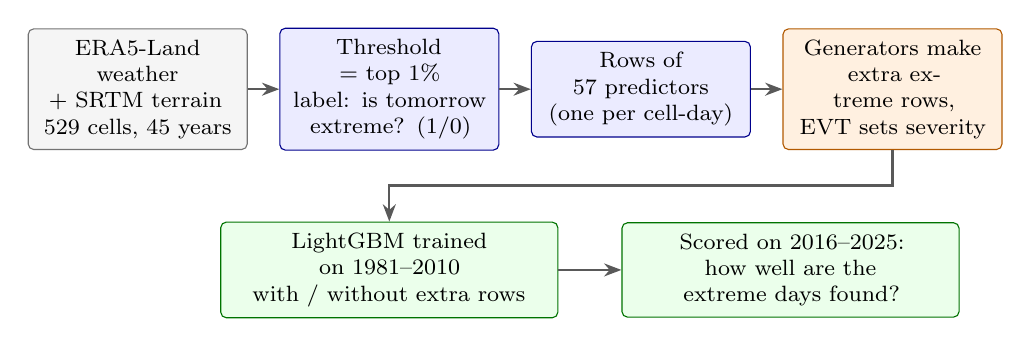
\begin{tikzpicture}[node distance=4mm]
\node[bdat,text width=2.5cm] (d) {ERA5-Land weather\\+ SRTM terrain\\529 cells, 45 years};
\node[blue box,text width=2.5cm,right=of d] (l) {Threshold = top 1\%\\label: is tomorrow\\extreme? (1/0)};
\node[blue box,text width=2.5cm,right=of l] (r) {Rows of\\57 predictors\\(one per cell-day)};
\node[orange box,text width=2.5cm,right=of r] (g) {Generators make\\extra extreme rows,\\EVT sets severity};
\node[green box,text width=4.0cm,below=9mm of l] (c) {LightGBM trained on 1981--2010\\with / without extra rows};
\node[green box,text width=4.0cm,right=8mm of c] (t) {Scored on 2016--2025:\\how well are the\\extreme days found?};
\draw[ar] (d) -- (l); \draw[ar] (l) -- (r); \draw[ar] (r) -- (g);
\draw[ar] (g.south) |- ++(0,-0.45) -| (c.north);
\draw[ar] (c) -- (t);
\end{tikzpicture}
\caption{The whole project in one picture.}
\end{figure}

\section*{The answer}
\begin{itemize}
  \item With real data only, the classifier scores \textbf{0.441} on the most severe days (PR-AUC, explained in
        Chapter~\ref{ch:metrics}; 1 is perfect).
  \item Adding extreme days from TVAE or CTGAN raises this to \textbf{0.601 (+36\%)}; from the diffusion model to
        \textbf{0.579 (+31\%)}.
  \item EVT is the reason it works: putting most added days in the rarest part of the tail improved every generator
        (by up to 14\%), while adding days without that focus helped much less.
\end{itemize}

\begin{sayit}
``Extreme heat days are 1\% of the data, so a model rarely sees them. I used generative models to create more of them,
and extreme value theory to make most of the new days the rare, severe kind, within physical limits. On years the
model never saw, this made its warnings for the most dangerous days 31 to 36\% better.''
\end{sayit}

% =============================================================================
\chapter{Weather and Climate of India}
\label{ch:climate}
% =============================================================================
This chapter gives the climate background needed for the rest of this guide: how weather differs across the
regions of India, which factors cause these differences, and where Himachal Pradesh fits.

\section{Weather Regions of India}
India stretches over about 30 degrees of latitude, from the equatorial south to the high Himalaya, so its weather
varies strongly from region to region. Two common ways of dividing it are used here.

\textbf{IMD homogeneous regions.} For monsoon monitoring and forecasting, IMD groups its meteorological subdivisions
into four broad regions with similar rainfall: Northwest India, Central India, South Peninsula, and East \& Northeast
India (Figure~\ref{fig:indiaregions}). Their normal June--September rainfall ranges from 587.6\,mm in Northwest India
to 1{,}367.3\,mm in East \& Northeast India. Himachal Pradesh belongs to \textbf{Northwest
India}, the driest of the four in the monsoon and the one most affected by winter western disturbances and pre-monsoon
heat.

\begin{figure}[H]
\centering
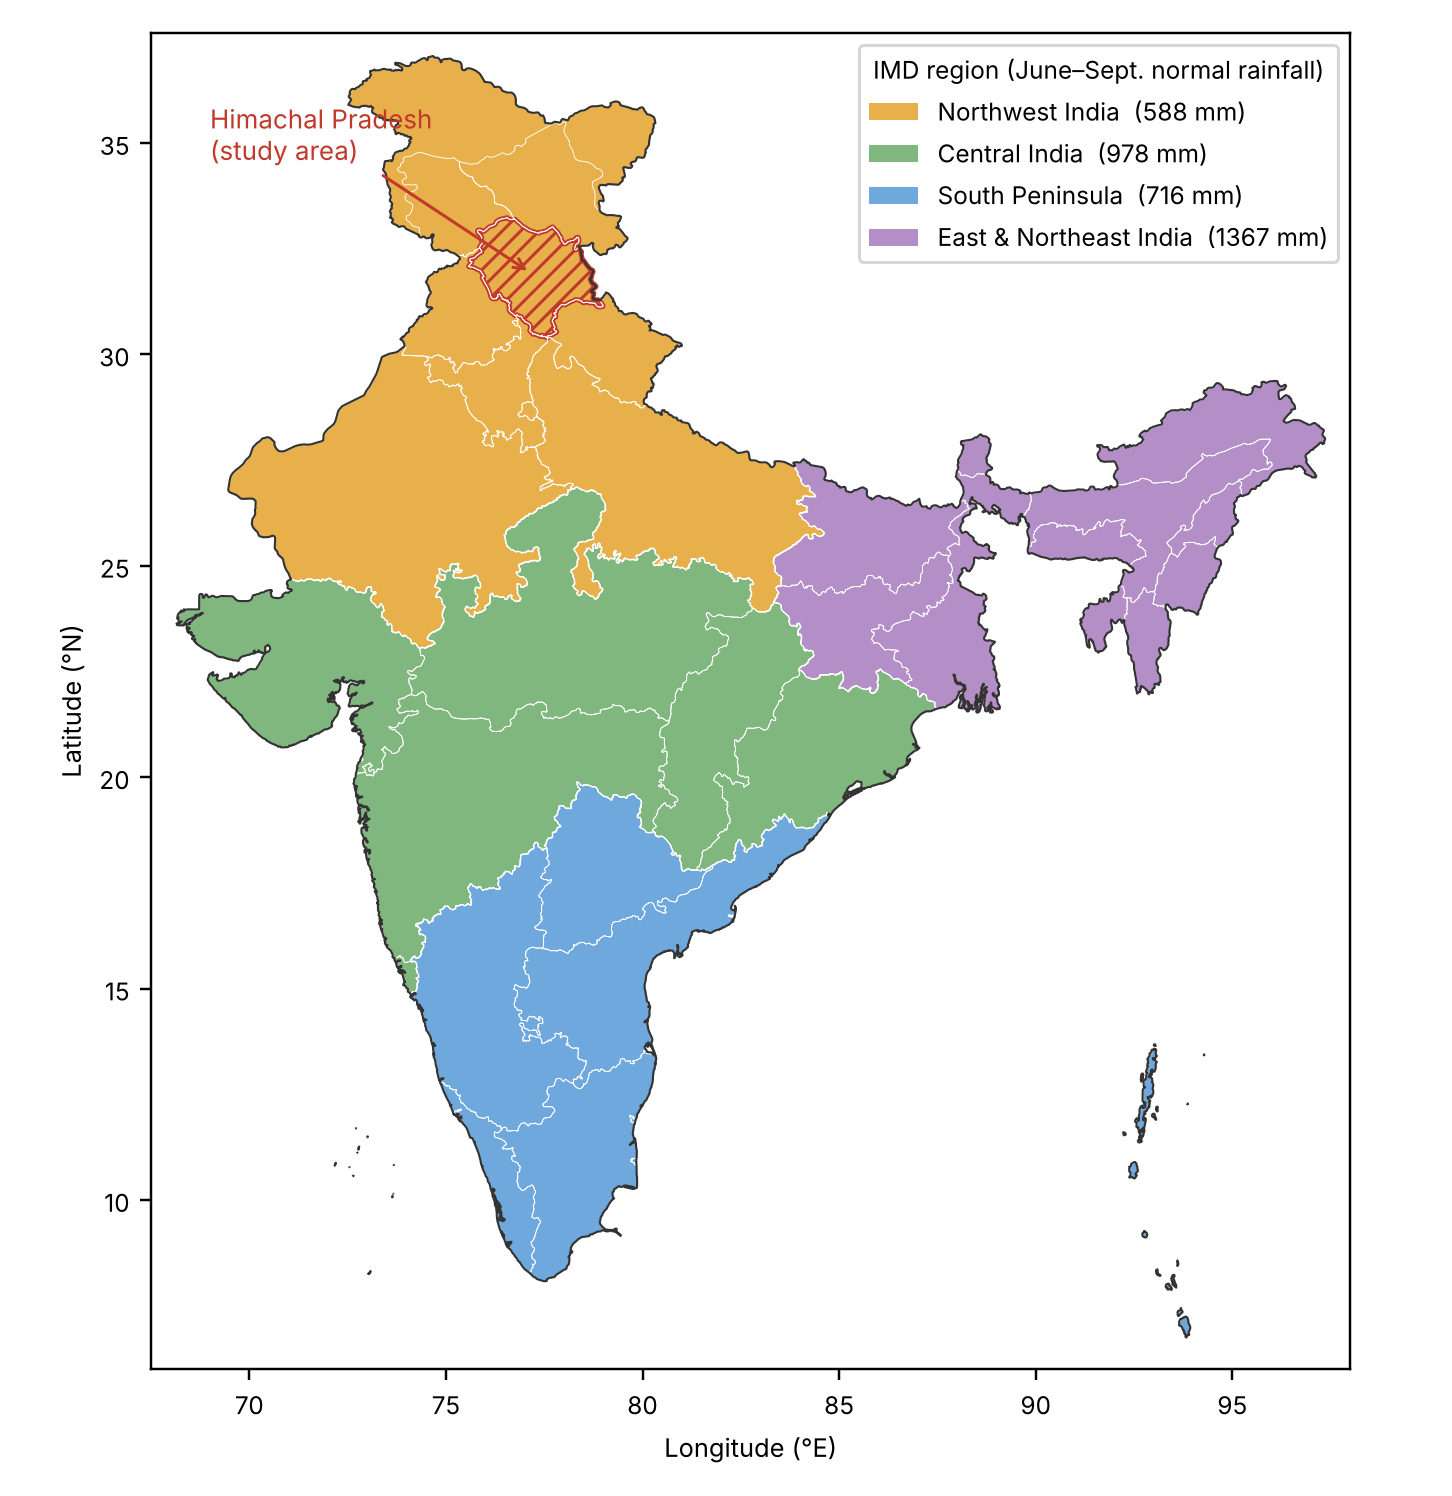
\includegraphics[width=0.74\textwidth]{fig_india_regions.png}
\caption{IMD's four homogeneous rainfall regions, drawn here by state, with their normal June--September rainfall
(1971--2020). IMD defines the regions by meteorological subdivision, so the state outlines are
an approximation. Himachal Pradesh, the study area, is hatched. Boundaries: Natural Earth (India's official view).}
\label{fig:indiaregions}
\end{figure}

\textbf{Climate types.} By temperature and rainfall, the country also falls into a few broad climate types
(Figure~\ref{fig:indiaclimate} and Table~\ref{tab:climtypes}).

\begin{figure}[H]
\centering
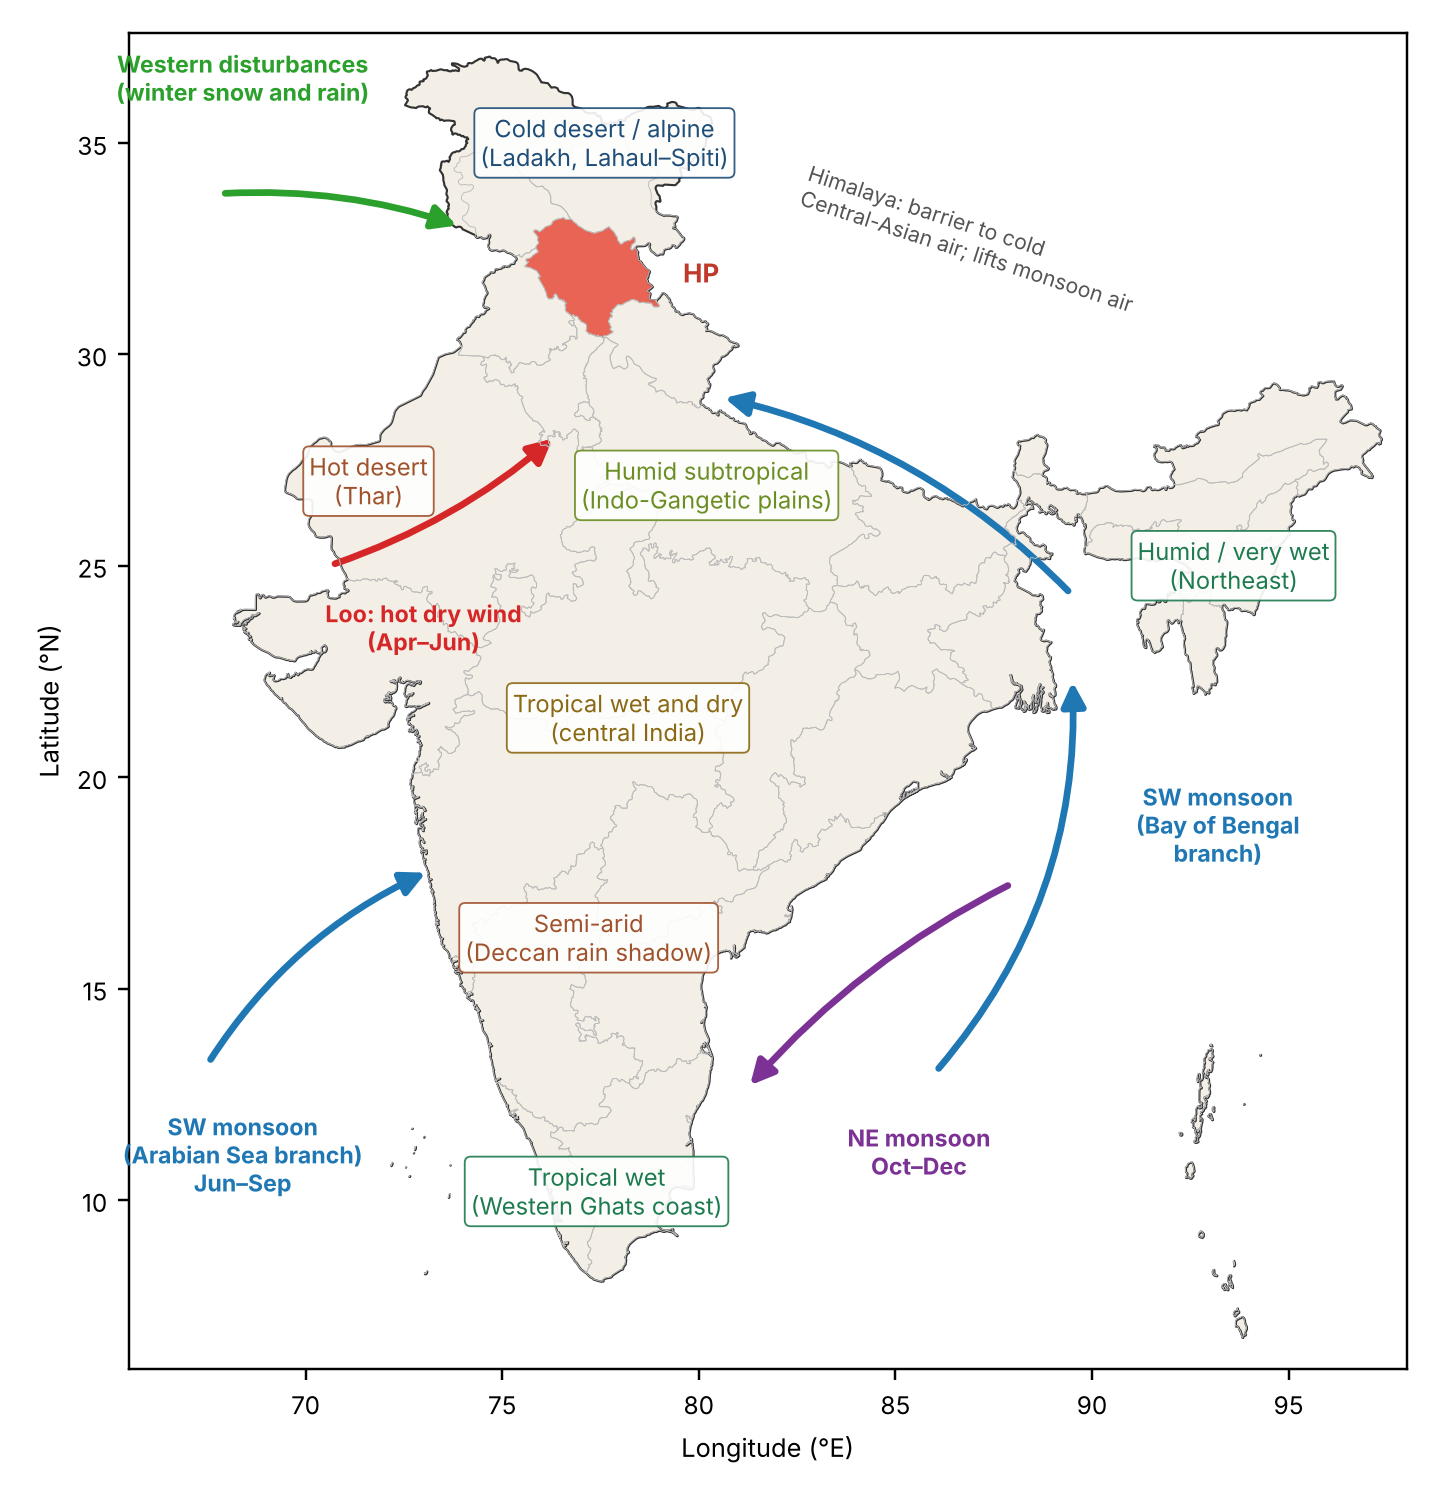
\includegraphics[width=0.74\textwidth]{fig_india_climate.png}
\caption{Broad climate types of India (labels placed at their typical location; no exact borders are implied) and
the main winds that shape them. Blue: the two branches of the southwest monsoon; purple: the northeast monsoon; green:
western disturbances; red: the hot \emph{loo} wind. Himachal Pradesh is shown in red.}
\label{fig:indiaclimate}
\end{figure}

\begin{table}[H]\footnotesize
\centering
\caption{Broad climate types of India.}
\label{tab:climtypes}
\begin{tabular}{|p{3.2cm}|p{4.2cm}|p{7.0cm}|}
\hline
\textbf{Climate type} & \textbf{Where} & \textbf{Main features}\\ \hline
Tropical wet & Western Ghats coast (Kerala, Konkan), parts of the Northeast & Hot and humid all year; very heavy
monsoon rain on slopes facing the wind.\\ \hline
Tropical wet and dry & Most of central and peninsular India & Hot summers, a clear wet season (monsoon) and a long dry
season.\\ \hline
Semi-arid & Interior Deccan (in the rain shadow of the Western Ghats), parts of Gujarat and Rajasthan & Low, unreliable
rain; hot summers.\\ \hline
Hot desert & Thar desert (western Rajasthan) & Very little rain; very hot days and cool nights; dust storms.\\ \hline
Humid subtropical & Indo-Gangetic plains, Himalayan foothills (including lower Himachal Pradesh) & Hot summers with
heatwaves, wet monsoon, cool to cold winters with fog.\\ \hline
Mountain (temperate to alpine) & Himalaya (middle and high Himachal Pradesh, Uttarakhand, Jammu \& Kashmir, Sikkim)
& Temperature falls with height; winter snow; climate changes over short distances.\\ \hline
Cold desert & Ladakh, Lahaul--Spiti and upper Kinnaur & Behind the main Himalayan ranges; very dry, very cold
winters, strong sunshine.\\ \hline
\end{tabular}
\end{table}

\section{Factors that Affect Weather in India}
The regional differences above come from a small set of physical factors (Figure~\ref{fig:factors}).

\begin{figure}[H]
\centering
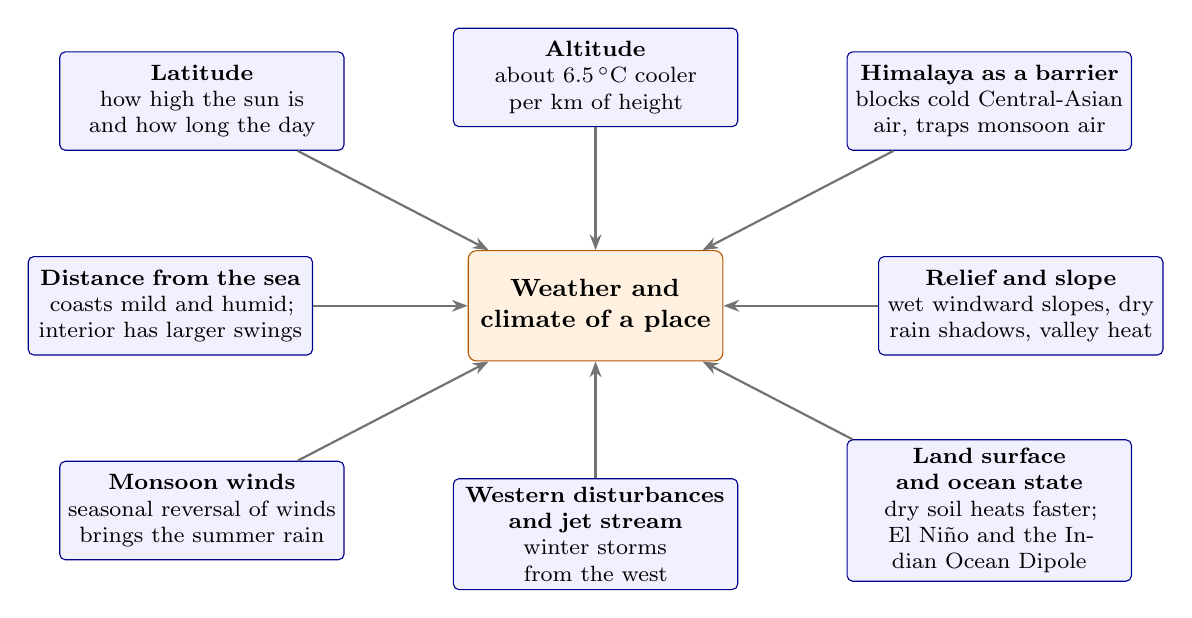
\begin{tikzpicture}[
  fac/.style={draw=blue!55!black,fill=blue!6,rounded corners=2pt,text width=3.4cm,align=center,font=\footnotesize,minimum height=1.25cm,inner sep=3pt},
  mid/.style={draw=orange!70!black,fill=orange!12,rounded corners=3pt,text width=3.0cm,align=center,font=\small\bfseries,minimum height=1.4cm},
  ar2/.style={-{Stealth[length=2mm]},thick,black!55}]
\node[mid] (c) at (0,0) {Weather and climate of a place};
\node[fac] (f1) at (-5.0, 2.6) {\textbf{Latitude}\\ how high the sun is and how long the day};
\node[fac] (f2) at (0, 2.9) {\textbf{Altitude}\\ about 6.5\,$^\circ$C cooler per km of height};
\node[fac] (f3) at (5.0, 2.6) {\textbf{Himalaya as a barrier}\\ blocks cold Central-Asian air, traps monsoon air};
\node[fac] (f4) at (-5.4, 0) {\textbf{Distance from the sea}\\ coasts mild and humid; interior has larger swings};
\node[fac] (f5) at (5.4, 0) {\textbf{Relief and slope}\\ wet windward slopes, dry rain shadows, valley heat};
\node[fac] (f6) at (-5.0,-2.6) {\textbf{Monsoon winds}\\ seasonal reversal of winds brings the summer rain};
\node[fac] (f7) at (0,-2.9) {\textbf{Western disturbances and jet stream}\\ winter storms from the west};
\node[fac] (f8) at (5.0,-2.6) {\textbf{Land surface and ocean state}\\ dry soil heats faster; El Ni\~no and the Indian Ocean Dipole};
\foreach \f in {f1,f2,f3,f4,f5,f6,f7,f8} \draw[ar2] (\f) -- (c);
\end{tikzpicture}
\caption{The main factors that control the weather and climate of a place in India.}
\label{fig:factors}
\end{figure}

\begin{enumerate}
\item \textbf{Latitude.} The Tropic of Cancer crosses the middle of India. The south is close to the equator and warm
all year; the north has a large difference between summer and winter.
\item \textbf{Altitude.} Air cools by about 6.5\,$^\circ$C for each kilometre of height on average. This is why the
same calendar day can be 40\,$^\circ$C in the plains and below freezing in the high Himalaya, and why this project
sets a separate threshold for every grid cell (Chapter~\ref{ch:extreme}).
\item \textbf{The Himalaya as a barrier.} The mountain wall keeps the cold, dry winter air of Central Asia out of
northern India, and in summer forces the moist monsoon winds to rise and release their rain on the southern slopes.
\item \textbf{Distance from the sea.} The sea warms and cools slowly, so coastal places have small daily and yearly
temperature ranges and high humidity. Inland places, far from the sea, have hotter summers and colder winters.
\item \textbf{Relief and slope (orographic effect).} When moist air is pushed up a mountain it cools, its water
vapour condenses and rain falls on the windward side; the air that comes down the other side is dry and warm, leaving
a \emph{rain shadow} (Figure~\ref{fig:orographic}). The Western Ghats and the Deccan, and the main Himalayan ranges
and Lahaul--Spiti, are two such pairs.
\item \textbf{Monsoon winds.} In summer the land heats much faster than the Indian Ocean; low pressure over north-west
India draws in moist south-westerly winds from the sea (the \emph{southwest monsoon}, with an Arabian Sea branch and a
Bay of Bengal branch). In winter the winds reverse and blow from the land (the \emph{northeast monsoon}), giving rain
only where they cross the Bay of Bengal, mainly in Tamil Nadu.
\item \textbf{Western disturbances and the jet stream.} In winter and spring, storms that form over the Mediterranean
region travel east along the subtropical westerly jet stream and bring snow and rain to the western Himalaya. They are
the main source of winter precipitation in Himachal Pradesh.
\item \textbf{Land surface and ocean state.} Dry soil uses less of the sun's energy for evaporation, so more of it
heats the air: dry spells before or during the summer make heat extremes more likely. On a larger scale, El Ni\~no
events in the Pacific and the Indian Ocean Dipole change the strength of the monsoon from year to year.
\end{enumerate}

\begin{figure}[H]
\centering
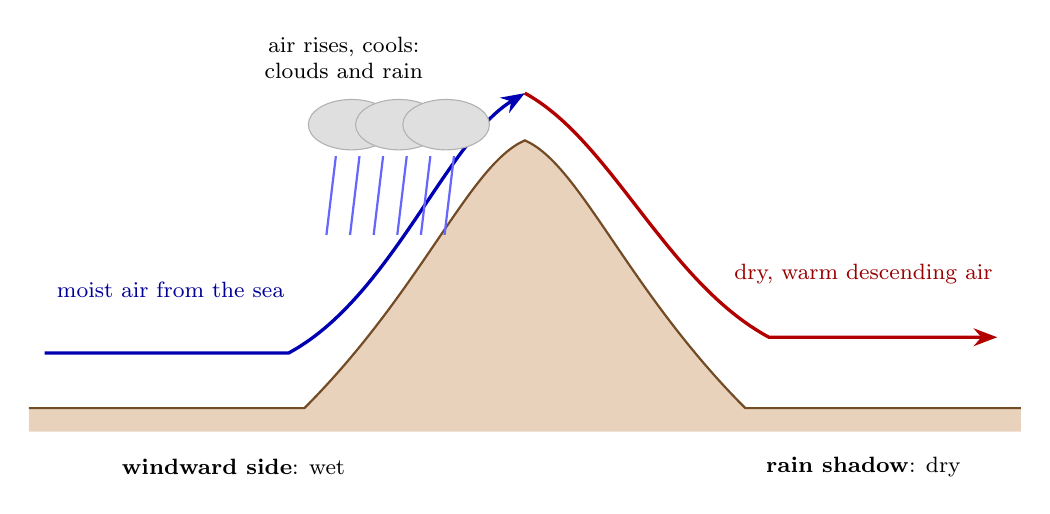
\begin{tikzpicture}[x=1cm,y=1cm]
\fill[brown!35] (0,0) -- (3.5,0) .. controls (5,1.5) and (5.6,3.1) .. (6.3,3.4) .. controls (7,3.1) and (7.6,1.5) .. (9.1,0) -- (12.6,0) -- (12.6,-0.3) -- (0,-0.3) -- cycle;
\draw[brown!60!black,thick] (0,0) -- (3.5,0) .. controls (5,1.5) and (5.6,3.1) .. (6.3,3.4) .. controls (7,3.1) and (7.6,1.5) .. (9.1,0) -- (12.6,0);
\draw[-{Stealth[length=3mm]},very thick,blue!70!black] (0.2,0.7) -- (3.3,0.7) .. controls (4.6,1.4) and (5.3,3.4) .. (6.3,4.0);
\draw[-{Stealth[length=3mm]},very thick,red!70!black] (6.3,4.0) .. controls (7.4,3.4) and (8.1,1.6) .. (9.4,0.9) -- (12.3,0.9);
\foreach \x in {4.1,4.7,5.3} \draw[fill=gray!25,draw=gray!60] (\x,3.6) ellipse (0.55 and 0.32);
\foreach \x in {3.9,4.2,4.5,4.8,5.1,5.4} \draw[blue!60,thick] (\x,3.2) -- (\x-0.12,2.2);
\node[font=\footnotesize,align=center,blue!60!black] at (1.8,1.5) {moist air from the sea};
\node[font=\footnotesize,align=center] at (4.0,4.45) {air rises, cools:\\clouds and rain};
\node[font=\footnotesize,align=center] at (2.6,-0.75) {\textbf{windward side}: wet};
\node[font=\footnotesize,align=center,red!60!black] at (10.6,1.7) {dry, warm descending air};
\node[font=\footnotesize,align=center] at (10.6,-0.75) {\textbf{rain shadow}: dry};
\end{tikzpicture}
\caption{The orographic effect: mountains make one side wet and the other dry.}
\label{fig:orographic}
\end{figure}

\section{Himachal Pradesh}
Himachal Pradesh lies in Northwest India on the southern side of the western Himalaya. Its height rises from about
300\,m near Una in the south-west to above 6{,}000\,m in the north-east, so it holds several climates within a short
distance. Using the elevation bands of the state's agro-climatic zones, the 529 grid cells of this project fall into
four groups (Figure~\ref{fig:hpzones}): 95 sub-tropical low-hill cells (below 1{,}000\,m), 47 sub-temperate mid-hill
cells (1{,}000--1{,}500\,m), 89 wet temperate high-hill cells (1{,}500--2{,}500\,m) and 298 dry temperate or cold-desert
cells (above 2{,}500\,m). More than half of the state therefore lies above 2{,}500\,m.

\begin{figure}[H]
\centering
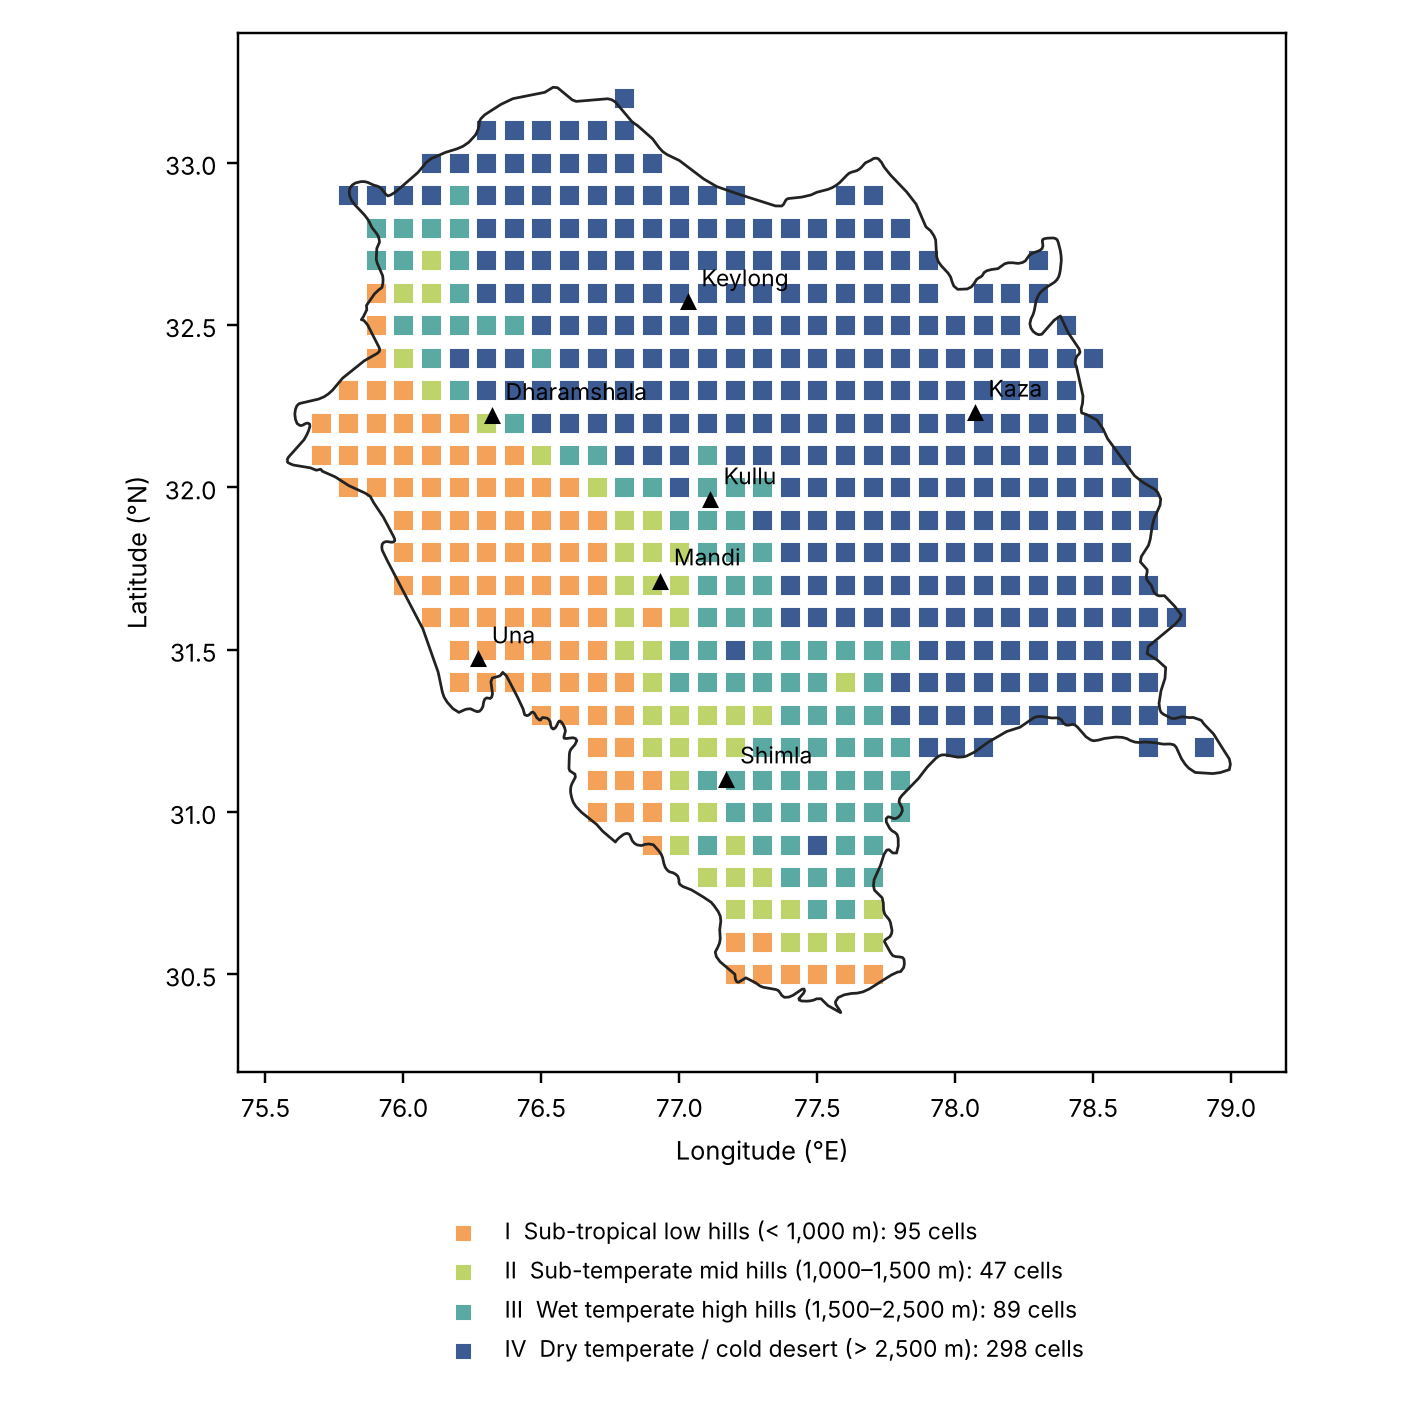
\includegraphics[width=0.66\textwidth]{fig_hp_zones.png}
\caption{The 529 grid cells of Himachal Pradesh coloured by elevation band (mean SRTM height of the cell). Triangles
mark towns for orientation.}
\label{fig:hpzones}
\end{figure}

\begin{itemize}
\item \textbf{Low hills (Una, Kangra valley, Bilaspur).} Hot pre-monsoon months with temperatures near those of the
Punjab plains, and a wet monsoon. Heatwaves from the plains reach here.
\item \textbf{Mid and high hills (Mandi, Shimla, Kullu).} Mild summers and cold winters with snow at higher places;
the heaviest monsoon rain falls on the outer ranges such as the Dhauladhar near Dharamshala.
\item \textbf{Cold desert (Lahaul--Spiti, upper Kinnaur).} Behind the Pir Panjal and Great Himalayan ranges, in their
rain shadow: little monsoon rain, snow mainly from western disturbances, very cold winters.
\end{itemize}

\textbf{Why this matters for the project.}
\begin{itemize}
\item The same temperature is ordinary in Una and extreme in Kaza, so a single national rule cannot describe extremes
everywhere. IMD itself uses different heatwave rules for plains (at least 40\,$^\circ$C) and hilly regions (at least
30\,$^\circ$C), together with a departure of 4.5\,$^\circ$C or more from normal. This project goes
one step further and uses the 99th percentile of each cell in each season (Chapter~\ref{ch:extreme}).
\item Seasons behave differently: pre-monsoon extremes are dry heat; monsoon extremes come in breaks of the monsoon;
winter extremes are warm spells between western disturbances. That is why thresholds and the EVT fit are computed per
season.
\item The factors above are what the predictors measure: elevation and slope (altitude and relief), soil moisture and
recent rain (land-surface dryness), humidity and dewpoint (monsoon moisture), surface pressure and its change
(passing disturbances) and solar radiation (clear skies).
\end{itemize}


\begin{sayit}
``India has four IMD rainfall regions; Himachal Pradesh is in Northwest India. Its weather is shaped by altitude, the
Himalaya, the monsoon and western disturbances. Because the state goes from 300\,m to over 6,000\,m, the same
temperature can be normal in Una and extreme in Kaza, so I define extremes per cell and per season.''
\end{sayit}

% =========================================================================
\chapter{The data}
\label{ch:data}
% =========================================================================

\section{Weather and climate}
\textbf{Weather} is the state of the air on a given day: how hot, how wet, how windy. \textbf{Climate} is the long-run
average of weather, and the range of what is normal, at a place. An \emph{extreme} is a day far outside that normal
range. This project predicts weather (tomorrow) but defines ``extreme'' using climate (the last 30 years).

\section{What a reanalysis is}
Weather stations are few in the mountains, and a station only tells you about one point. A \textbf{reanalysis} solves
this by running a computer weather model over past decades and, every few hours, correcting it with all available real
observations (stations, satellites, weather balloons, aircraft). The result is a complete map of past weather on a
regular grid, with a value for every place and every hour, even where nobody measured.

\begin{figure}[H]
\centering
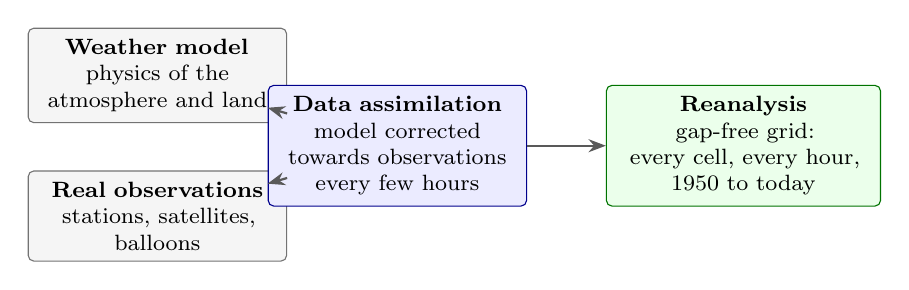
\begin{tikzpicture}[node distance=6mm]
\node[bdat,text width=3.0cm] (m) {\textbf{Weather model}\\physics of the\\atmosphere and land};
\node[bdat,text width=3.0cm,below=of m] (o) {\textbf{Real observations}\\stations, satellites,\\balloons};
\node[blue box,text width=3.0cm,right=14mm of $(m)!0.5!(o)$] (a) {\textbf{Data assimilation}\\model corrected\\towards observations\\every few hours};
\node[green box,text width=3.2cm,right=10mm of a] (r) {\textbf{Reanalysis}\\gap-free grid:\\every cell, every hour,\\1950 to today};
\draw[ar] (m) -- (a); \draw[ar] (o) -- (a); \draw[ar] (a) -- (r);
\end{tikzpicture}
\caption{How a reanalysis is made.}
\end{figure}

\textbf{Strength:} no gaps, long record, many variables. \textbf{Weakness:} it is a model reconstruction, not a direct
measurement, so it can be biased, especially in steep mountains where the model's terrain is smoother than reality.

\section{ERA5-Land}
ERA5-Land is the reanalysis used in this project. It is made by the \emph{European Centre for Medium-Range Weather
Forecasts} (ECMWF) for the EU's \emph{Copernicus Climate Change Service}, and is free from the Copernicus Climate Data
Store.
\begin{itemize}
  \item \textbf{Grid:} $0.1^\circ$ of latitude and longitude, about 9\,km. (ERA5, its parent, is 0.25$^\circ$, about
        28\,km.)
  \item \textbf{Time:} hourly, 1950 to a few days ago. The project uses daily values for 1981--2025.
  \item \textbf{Daily statistics:} from the 24 hourly values of a day, ERA5-Land gives the daily maximum, minimum and
        mean. The project uses the raw values (no bias correction).
  \item \textbf{Why chosen:} it was the only free data set that is long (45 years), fine enough for mountains, gap-free
        and has many variables. Other data sets were too coarse (ERA5, IMD gridded, MERRA-2, CMIP6), stopped too early
        (IMDAA ends 2018) or had too few points (only 3 usable GSOD weather stations in the state).
\end{itemize}

\section{The grid and the 529 cells}
\begin{example}[Where 529 comes from]
\begin{enumerate}[leftmargin=*]
  \item Data were downloaded for the box 30.3--33.3$^\circ$N, 75.5--79.1$^\circ$E.
  \item At $0.1^\circ$ spacing: latitude 30.3, 30.4, \dots, 33.3 gives 31 rows; longitude 75.5, \dots, 79.1 gives 37
        columns; $31\times37=1{,}147$ cells.
  \item Keep a cell only if its centre lies inside the state boundary (GADM outline): \textbf{529 cells}.
  \item Check: one cell at 32$^\circ$N is $11.1\,\text{km}$ (north--south) $\times$ $9.4\,\text{km}$ (east--west,
        shorter because longitude lines converge), about 105\,km$^2$. $529\times105\approx55{,}500$\,km$^2$, close to
        Himachal's area of about 55{,}700\,km$^2$.
\end{enumerate}
\end{example}

\begin{figure}[H]
\centering
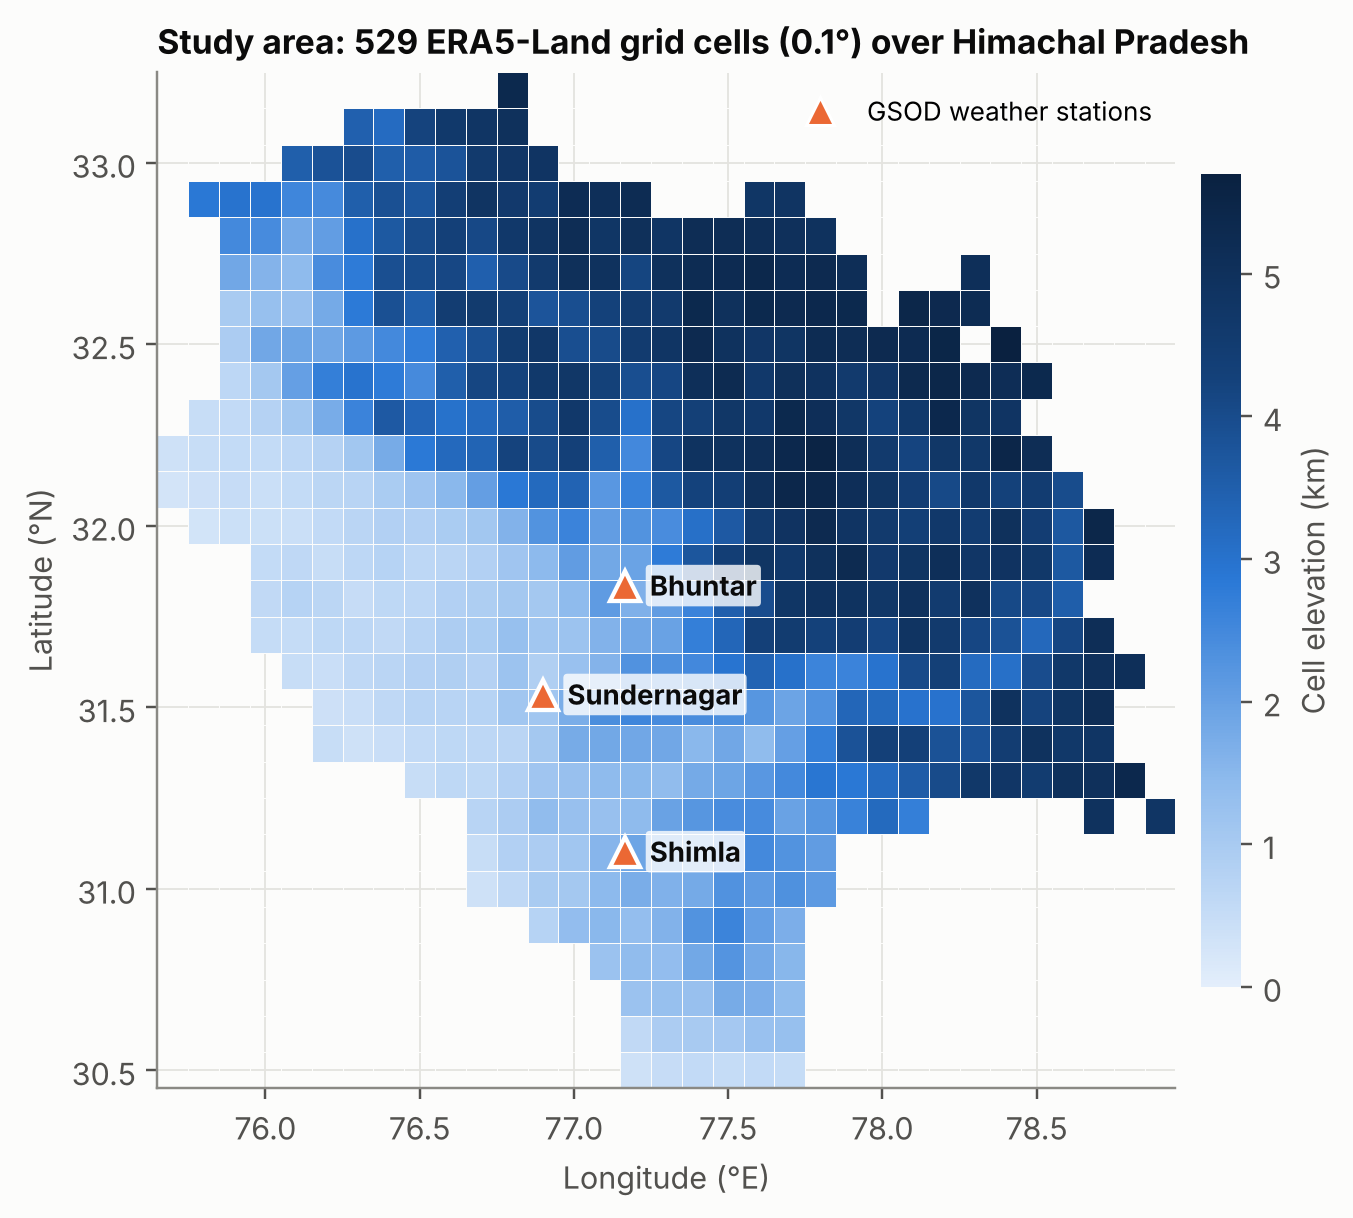
\includegraphics[width=0.62\textwidth]{fig_study_area.png}
\caption{The 529 cells coloured by elevation, and the three GSOD weather stations (kept for future checks).}
\end{figure}

\section{SRTM terrain}
SRTM (Shuttle Radar Topography Mission) is a map of ground height measured by radar from the Space Shuttle
\emph{Endeavour} in February 2000 (NASA). It gives a height every 30\,m. For each grid cell, the 30\,m heights were
averaged to give the cell's \textbf{mean elevation} (m), and the local slopes were averaged to give its \textbf{mean
slope} (degrees). These two numbers do not change with time; they tell the model whether a cell is a low valley or a
high, steep ridge.

\section{The variables and why each matters for heat}
\begin{table}[H]
\centering
\caption{Variables used. All except relative humidity come from ERA5-Land.}
\footnotesize
\begin{tabularx}{\textwidth}{>{\raggedright\arraybackslash}p{3.2cm}>{\raggedright\arraybackslash}p{1.4cm}>{\raggedright\arraybackslash}p{1.4cm}X}
\toprule
\textbf{Variable} & \textbf{Code} & \textbf{Unit} & \textbf{What it means and why it matters}\\
\midrule
Air temperature at 2\,m: daily max, min, mean & \texttt{t2m\_max}, \texttt{t2m\_min}, \texttt{t2m\_mean} & $^\circ$C
  & Temperature of the air at head height. The daily maximum defines the extreme day.\\
Dewpoint at 2\,m & \texttt{d2m} & $^\circ$C & The temperature at which the air would become saturated; higher means
  more moisture in the air.\\
Relative humidity & \texttt{rh} & \% & How close the air is to saturation, computed from temperature and dewpoint.
  Dry air heats faster.\\
Surface pressure & \texttt{sp} & hPa & Weight of the air above. Rising pressure usually means settled, clear, sunny
  weather.\\
Solar radiation down & \texttt{ssrd} & W\,m$^{-2}$ & Sunshine reaching the ground; the energy that heats it.\\
Soil water, top 7\,cm & \texttt{swvl1} & m$^3$\,m$^{-3}$ & Share of the soil volume that is water. Wet soil uses
  sunshine to evaporate water; dry soil turns it into heat.\\
Total precipitation & \texttt{tp} & mm & Rain (and melted snow) per day. Rain cools; dry spells come before heat.\\
Mean elevation, mean slope & \texttt{elev\_m}, \texttt{slope\_deg} & m, $^\circ$ & From SRTM. Temperature falls
  about 6.5\,$^\circ$C per km of height.\\
\bottomrule
\end{tabularx}
\end{table}

\textbf{Unit conversions done:} temperature K $\to$ $^\circ$C ($-273.15$), pressure Pa $\to$ hPa ($\div100$), rain
m $\to$ mm ($\times1000$), radiation J\,m$^{-2}$ per day $\to$ W\,m$^{-2}$ ($\div86{,}400$). Rain and radiation are
\emph{accumulated} in ERA5-Land: the value stamped at midnight of day $D+1$ is the total for day $D$, so they were moved
back one day.

\section{Seasons}
The India Meteorological Department (IMD) divides the year into four seasons, used throughout the project:
\begin{center}
\begin{tabular}{llc}
\toprule
\textbf{Season} & \textbf{Months} & \textbf{Days}\\
\midrule
Winter & December, January, February & about 90\\
Pre-monsoon & March, April, May & 92\\
Monsoon & June, July, August, September & 122\\
Post-monsoon & October, November & 61\\
\bottomrule
\end{tabular}
\end{center}

\begin{sayit}
``I used ERA5-Land, a reanalysis from ECMWF: a weather model corrected with real observations, giving gap-free daily
weather on a 9\,km grid. Inside Himachal that is 529 cells for 45 years. Height and slope of each cell come from NASA's
SRTM terrain map.''
\end{sayit}

% =========================================================================
\chapter{What is an extreme heat day?}
\label{ch:extreme}
% =========================================================================

\section{Percentiles}
Sort a list of values from smallest to largest. The \textbf{$p$-th percentile} is the value below which $p$\% of them
lie. The 99th percentile is the value that only 1\% of the list exceeds.

\begin{example}[A small example]
Take the daily maximum temperatures of 1{,}000 summer days at one cell, sorted. The 99th percentile is (about) the
990th value: only 10 days, 1\%, were hotter. If that value is 33.4\,$^\circ$C, then 33.4\,$^\circ$C is the threshold.
\end{example}

\section{The threshold $u$}
For every \textbf{cell} $c$ and every \textbf{season} $g$, the threshold $u_{c,g}$ is the 99th percentile of the daily
maximum temperature of that cell in that season, using only the years \textbf{1981--2010}.
\begin{itemize}
  \item $529\text{ cells}\times4\text{ seasons}=\textbf{2{,}116 thresholds}$.
  \item A day is an \textbf{extreme heat day} if its maximum temperature is above the threshold of its cell and season:
        $T^{\max}_{c,t}>u_{c,g(t)}$.
  \item By construction, about 1\% of the days of 1981--2010 are extreme in every cell and season.
\end{itemize}

\begin{figure}[H]
\centering
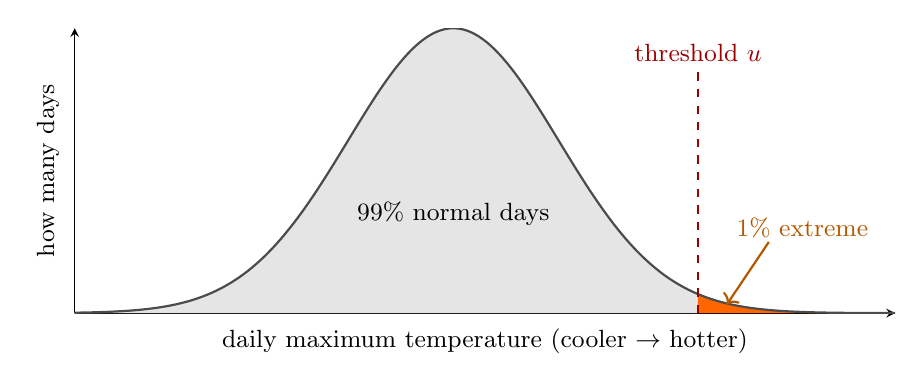
\begin{tikzpicture}
\begin{axis}[width=12cm,height=5.2cm,axis lines=left,xlabel={daily maximum temperature (cooler $\rightarrow$ hotter)},
  ylabel={how many days},xtick=\empty,ytick=\empty,ymin=0,xmin=-3.6,xmax=4.2,samples=200,domain=-3.6:4.2,
  xlabel style={font=\small},ylabel style={font=\small}]
\addplot[fill=black!10,draw=none,domain=-3.6:2.326] {exp(-x^2/2)} \closedcycle;
\addplot[fill=orange!80!red,draw=none,domain=2.326:4.2] {exp(-x^2/2)} \closedcycle;
\addplot[thick,black!70] {exp(-x^2/2)};
\draw[dashed,thick,red!60!black] (axis cs:2.326,0) -- (axis cs:2.326,0.85);
\node[font=\small,red!60!black,anchor=south] at (axis cs:2.326,0.85) {threshold $u$};
\node[font=\small] at (axis cs:0,0.35) {99\% normal days};
\node[font=\small,orange!70!black,anchor=west] at (axis cs:2.6,0.3) {1\% extreme};
\draw[->,orange!70!black,thick] (axis cs:3.0,0.25) -- (axis cs:2.6,0.03);
\end{axis}
\end{tikzpicture}
\caption{All days of one cell and season, from cooler to hotter. Days beyond the threshold (orange) are extreme heat
days. The real shape is not exactly a bell curve; this is only a picture of the idea of a ``tail''.}
\end{figure}

\section{Why a threshold per cell and per season?}
\begin{itemize}
  \item \textbf{Per cell:} 30\,$^\circ$C is a normal summer day in the plains but extreme high up. Each cell is compared
        with its own past. Thresholds fall by 6--7\,$^\circ$C per km of altitude.
  \item \textbf{Per season:} an unusually warm winter day is also an extreme, even though it is cooler than a normal
        summer day.
  \item \textbf{Fixed past (1981--2010):} the thresholds never change, so a warming climate shows up as more extreme days.
\end{itemize}

\section{The label}
The prediction is always about \textbf{tomorrow}. Call today day $D$. The label of a row is
\[
  \text{label}=\begin{cases}1 & \text{if day }D+1\text{ is an extreme heat day in this cell,}\\ 0 & \text{otherwise.}\end{cases}
\]
This is a \textbf{binary classification} problem: the answer is one of two classes, 1 (``extreme'') or 0 (``normal'').

\section{Normal and anomaly}
The \textbf{normal} of a cell for a calendar day is the 1981--2010 average maximum temperature over the 15 days centred
on that date (7 days either side). The \textbf{anomaly} of a day is its temperature minus its normal: $+3$ means 3
degrees warmer than usual for that date.

\section{The climate signal}
With the same fixed thresholds, extreme days were \textbf{1.02\%} of cell-days in 1981--2010 but \textbf{1.94\%} in
2016--2025: almost twice as many. This is also why a model that never warns is 99\% accurate in the old years but only
98\% accurate in the test years.

\begin{sayit}
``A day is extreme if it is hotter than 99\% of that cell's own days in the same season over 1981--2010. That gives
2,116 thresholds, and the task is: will tomorrow be above the threshold here, yes or no?''
\end{sayit}

% =========================================================================
\chapter{From days to rows: the 57 predictors}
\label{ch:rows}
% =========================================================================

\section{What a row is}
The classifier reads a \textbf{table}. One \textbf{row} is one cell on one day (a \emph{cell-day}); its columns are the
\textbf{predictors} (also called features or inputs) plus the label. A year gives about $529\times365\approx193{,}000$
rows. The classifier does not read a sequence of days, so the past must be written into the columns of the row: that is
why there are columns for yesterday, the day before, and summaries of the last weeks.

\begin{figure}[H]
\centering
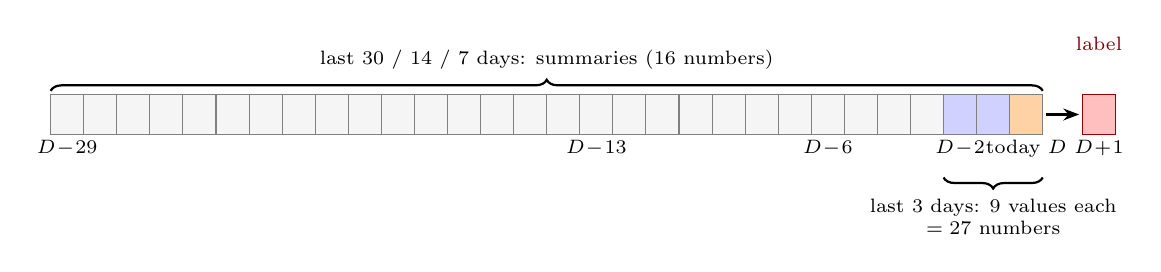
\begin{tikzpicture}[x=0.42cm,y=0.5cm,
  dbox/.style={draw=black!50,fill=#1,minimum height=0.5cm,minimum width=0.42cm,inner sep=0}]
\foreach \i in {0,...,29} { \node[dbox=black!4] at (\i,0) {}; }
\foreach \i in {27,28} { \node[dbox=blue!18] at (\i,0) {}; }
\node[dbox=orange!35] at (29,0) {};
\node[dbox=red!25,draw=red!60!black] at (31.2,0) {};
\node[font=\scriptsize,below] at (0,-0.4) {$D\!-\!29$};
\node[font=\scriptsize,below] at (16,-0.4) {$D\!-\!13$};
\node[font=\scriptsize,below] at (23,-0.4) {$D\!-\!6$};
\node[font=\scriptsize,below] at (27,-0.4) {$D\!-\!2$};
\node[font=\scriptsize,below] at (29,-0.4) {today $D$};
\node[font=\scriptsize,below] at (31.2,-0.4) {$D\!+\!1$};
\draw[decorate,decoration={brace,amplitude=4pt},thick] (-0.5,0.6) -- (29.5,0.6) node[midway,above=4pt,font=\scriptsize]{last 30 / 14 / 7 days: summaries (16 numbers)};
\draw[decorate,decoration={brace,amplitude=4pt,mirror},thick] (26.5,-1.6) -- (29.5,-1.6) node[midway,below=4pt,font=\scriptsize,align=center]{last 3 days: 9 values each\\$=27$ numbers};
\node[font=\scriptsize,align=center,red!50!black] at (31.2,1.8) {label};
\draw[-{Stealth[length=2mm]},thick] (29.6,0) -- (30.6,0);
\end{tikzpicture}
\caption{The days one row looks at. Only days up to today are used; nothing from tomorrow except the label.}
\end{figure}

\section{The five groups of predictors}
\begin{table}[H]
\centering
\caption{The 57 predictors grouped. The full list with units is Table 6 of the report.}
\footnotesize
\begin{tabularx}{\textwidth}{>{\raggedright\arraybackslash}p{3.3cm}c>{\raggedright\arraybackslash}X}
\toprule
\textbf{Group} & \textbf{How many} & \textbf{What is in it}\\
\midrule
A. Place & 4 & latitude, longitude, mean elevation, mean slope\\
B. Last three days & 27 & 9 daily values (max, min and mean temperature, dewpoint, humidity, pressure, sunshine, soil
  water, rain) for today, yesterday and the day before: $9\times3$\\
C. Today vs.\ normal & 2 & today's maximum and minimum temperature minus their normal\\
D. Last 1--4 weeks & 16 & average warmth over 7/14/30 days (5), length of the current warm spell, days since the last
  extreme, number of extremes in 30 days, rain over 7/30 days (2), soil water over 14/30 days (2), soil drying over 14
  days, average dewpoint and sunshine over 7 days (2), pressure change over 3 days\\
E. Gap to tomorrow's threshold & 8 & how far the last three days' maximum temperatures are from tomorrow's threshold, in
  $^\circ$C (3) and in units of the cell's variability (3), whether the gap is closing, and today's change in
  temperature\\
\midrule
\textbf{Total} & \textbf{57} & $4+27+2+16+8$\\
\bottomrule
\end{tabularx}
\end{table}

\begin{example}[Reading one row: Mandi, tomorrow]
To predict whether tomorrow will be extreme at the cell containing Mandi, the row contains: where the cell is and how
high it is (A); today's, yesterday's and the day before's weather there (B); whether today is warmer than usual for the
date (C); whether the last month has been hot and dry, how long the warm spell has lasted, and when the last extreme was
(D); and how close today's temperature already is to Mandi's own threshold for tomorrow's season (E). The model answers
with a probability that tomorrow is extreme.
\end{example}

\textbf{Why group E matters most:} if today is already only 0.5\,$^\circ$C below the threshold and warming, tomorrow
crossing it is likely. LightGBM is told that a smaller gap can never mean a \emph{lower} risk (a ``monotone
constraint'', Chapter~\ref{ch:clf}).

\section{Training, validation and test: splitting by time}
\begin{figure}[H]
\centering
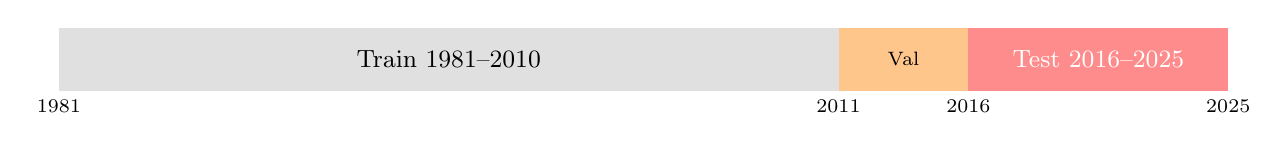
\begin{tikzpicture}[x=0.33cm]
\fill[black!12] (0,0) rectangle (30,0.8); \node[font=\small] at (15,0.4) {Train 1981--2010};
\fill[orange!45] (30,0) rectangle (35,0.8); \node[font=\scriptsize] at (32.5,0.4) {Val};
\fill[red!45] (35,0) rectangle (45,0.8); \node[font=\small,white] at (40,0.4) {Test 2016--2025};
\foreach \x/\y in {0/1981,30/2011,35/2016,45/2025} \node[font=\scriptsize,below] at (\x,0) {\y};
\end{tikzpicture}
\caption{The data are split by year, never at random.}
\end{figure}

\begin{center}
\footnotesize
\begin{tabular}{llrrl}
\toprule
\textbf{Part} & \textbf{Years} & \textbf{Rows} & \textbf{Extreme rows} & \textbf{Used for}\\
\midrule
Train & 1981--2010 & 2{,}889{,}927 & 29{,}604 (1.02\%) & fitting the classifier and the generators\\
Validation & 2011--2015 & 965{,}954 & 9{,}626 (1.00\%) & every choice (when to stop, warning cut-off)\\
Test & 2016--2025 & 1{,}932{,}437 & 37{,}450 (1.94\%) & the final scores, used once\\
\bottomrule
\end{tabular}
\end{center}

\begin{itemize}
  \item \textbf{Why by time?} Weather on neighbouring days is similar. A random split would put Monday in training
        and Tuesday in test, and the model would look better than it really is (\emph{data leakage}). Splitting by
        year is how a real forecast works: learn from the past, predict the future.
  \item \textbf{Why a random half of 1981--2010?} To fit in the memory of free Google Colab. It still keeps all 29{,}604
        extreme rows of that half.
  \item \textbf{Why a validation period?} If choices were made on the test years, the test score would be too
        optimistic. Validation is a separate ``practice exam''.
\end{itemize}

\begin{sayit}
``LightGBM reads a table, so the past is flattened into 57 columns: the place, the last three days of weather, the last
one to four weeks, and how far today is from tomorrow's threshold. I split by year: train 1981--2010, choose settings
on 2011--2015, test once on 2016--2025.''
\end{sayit}

% =========================================================================
\chapter{Why rare days are hard: imbalanced classification}
\label{ch:imb}
% =========================================================================

\section{Class imbalance}
A data set is \textbf{imbalanced} when one class is much rarer than the other. Here the rare (\emph{minority}) class,
extreme days, is about 1\% of training rows; the common (\emph{majority}) class, normal days, is 99\%. For every
extreme row the model sees 99 normal ones.

\section{The accuracy trap}
\textbf{Accuracy} is the share of all predictions that are right. In the test years 98.06\% of days are normal, so a
``model'' that \emph{never} warns is 98\% accurate and completely useless: it catches no extreme day. That is why the
project never judges models by accuracy (Chapter~\ref{ch:metrics}).

\section{What goes wrong in training}
A classifier learns by reducing its total error. Getting all normal days right already makes the error tiny, so the
few extreme days have little influence. Within the extremes, the \emph{most severe} days are rarer still (only a few
hundred in 30 years), so they are the worst learned, although they are the most dangerous.

\section{Standard fixes, and their limits}
\begin{itemize}
  \item \textbf{Class weights:} count each extreme row as if it were many rows. Does not add new information.
  \item \textbf{Random oversampling:} repeat real extreme rows. The model may memorise them (overfitting).
  \item \textbf{SMOTE} (Synthetic Minority Over-sampling Technique): make a new rare row on the straight line between
        a real rare row and one of its nearest rare neighbours. Variants: Borderline-SMOTE (only near the class
        boundary) and ADASYN (more where the class is hard).
\end{itemize}

\begin{figure}[H]
\centering
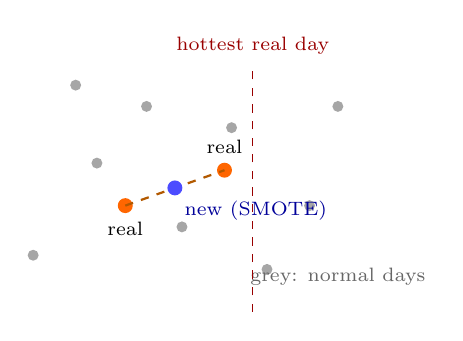
\begin{tikzpicture}[scale=0.9]
\foreach \p in {(0.3,0.5),(1.2,1.8),(2.4,0.9),(3.1,2.3),(0.9,2.9),(4.2,1.2),(3.6,0.3),(1.9,2.6),(4.6,2.6)}
  \fill[black!35] \p circle (2.2pt);
\fill[orange!80!red] (1.6,1.2) circle (3pt); \fill[orange!80!red] (3.0,1.7) circle (3pt);
\draw[dashed,orange!70!black,thick] (1.6,1.2) -- (3.0,1.7);
\fill[blue!70] (2.3,1.45) circle (3pt);
\node[font=\scriptsize,anchor=north] at (1.6,1.1) {real};
\node[font=\scriptsize,anchor=south] at (3.0,1.8) {real};
\node[font=\scriptsize,blue!60!black,anchor=north west] at (2.3,1.4) {new (SMOTE)};
\node[font=\scriptsize,black!60] at (4.6,0.2) {grey: normal days};
\draw[dashed,red!60!black] (3.4,-0.3) -- (3.4,3.2); \node[font=\scriptsize,red!60!black,anchor=south] at (3.4,3.2) {hottest real day};
\end{tikzpicture}
\caption{SMOTE places a new rare point between two real ones. It can never create a day hotter than the hottest real
one (dashed line), and it knows nothing about the physics of extremes.}
\end{figure}

\section{The idea of this project}
Instead of copying or interpolating, \textbf{learn} what extreme days look like with a \emph{generative model}
(Chapter~\ref{ch:gen}), and use \textbf{extreme value theory} (Chapter~\ref{ch:evt}) to decide how severe the new days
should be, so that most go to the thinnest, hottest part of the tail without passing what is physically possible.

\begin{sayit}
``Only 1 day in 100 is extreme, so a model that never warns is 98\% accurate and useless. Usual fixes reweight or copy
the rare days, or interpolate between them like SMOTE, which can't go beyond the hottest real day. So I generate new
extreme days instead, and let extreme value theory decide where in the tail to put them.''
\end{sayit}

% =========================================================================
\chapter{Extreme value theory (EVT)}
\label{ch:evt}
% =========================================================================

\section{Why a special theory for extremes}
Ordinary statistics (mean, standard deviation, normal curve) describe the \emph{typical} values, where almost all data
lie. The \textbf{tail}, the far end with the rare extremes, has very few points, and a curve fitted to all the data
usually gets the tail wrong. \textbf{Extreme value theory} is the branch of statistics that models only the tail.

\begin{keyidea}[In one line]
Model the tail, not the average.
\end{keyidea}

\section{Two ways to do EVT}
\begin{center}
\footnotesize
\begin{tabular}{p{3.2cm}p{5.2cm}p{2.6cm}c}
\toprule
\textbf{Approach} & \textbf{Data it uses} & \textbf{Distribution} & \textbf{Used here?}\\
\midrule
Block maxima & the single largest value of each block (e.g.\ hottest day of each year) & GEV (generalised extreme
  value) & No\\
\textbf{Peaks over threshold} & \textbf{every value above a high threshold} & \textbf{GPD (generalised Pareto)} &
  \textbf{Yes}\\
\bottomrule
\end{tabular}
\end{center}
Peaks over threshold uses every extreme day, not just one per year, so it gets more information from the same record.

\section{Threshold, exceedance and excess}
\begin{itemize}
  \item \textbf{Threshold $u$:} the 99th percentile of the cell and season (Chapter~\ref{ch:extreme}). \emph{We chose}
        this value; the theory only asks that it be high.
  \item \textbf{Exceedance:} a day above $u$, i.e.\ an extreme day.
  \item \textbf{Excess:} how far above, $T^{\max}-u$, in $^\circ$C.
\end{itemize}

\section{Standardising: the severity $z$}
An excess of 2\,$^\circ$C is huge in a calm valley cell and ordinary in a variable mountain cell. So each excess is
divided by $s$, the cell's own day-to-day spread (the standard deviation of its daily temperature anomaly in that
season):
\[
  z=\frac{T^{\max}-u}{s}.
\]
Now all 529 cells are on one scale, and one curve per season can be fitted to all of them together. $z$ is the
\textbf{severity} of an extreme day: 0 means just over the threshold, larger means more severe.

\section{The generalised Pareto distribution (GPD)}
\begin{keyidea}[The theorem behind EVT (Pickands--Balkema--de Haan)]
Whatever the original data look like, the excesses above a high enough threshold follow (approximately) a
\textbf{generalised Pareto distribution}.
\end{keyidea}

The chance that the severity is larger than $z$ is
\[
  P(Z>z)=\Big(1+\frac{\xi z}{\sigma}\Big)^{-1/\xi},\qquad z\ge0,
\]
with two numbers to fit: the \textbf{scale} $\sigma$ (the typical size of an excess) and the \textbf{shape} $\xi$
(``xi''), which decides the kind of tail.

\begin{figure}[H]
\centering
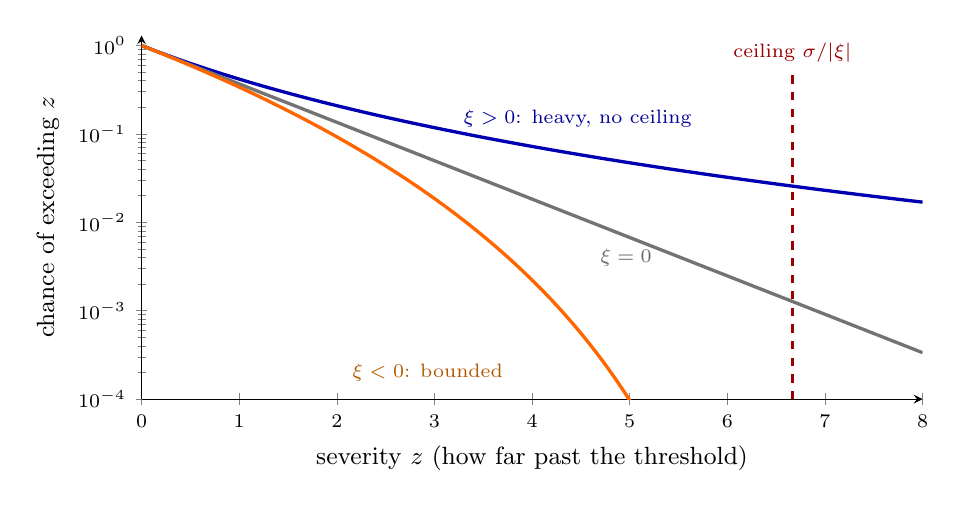
\begin{tikzpicture}
\begin{semilogyaxis}[width=11.5cm,height=6.2cm,axis lines=left,xmin=0,xmax=8,ymin=1e-4,ymax=1.3,
  xlabel={severity $z$ (how far past the threshold)},ylabel={chance of exceeding $z$},
  xlabel style={font=\small},ylabel style={font=\small},tick label style={font=\scriptsize},samples=300]
\addplot[very thick,blue!70!black,domain=0:8] {(1+0.3*x)^(-1/0.3)};
\addplot[very thick,black!55,domain=0:8] {exp(-x)};
\addplot[very thick,orange!80!red,domain=0:6.6] {(1-0.15*x)^(1/0.15)};
\draw[dashed,thick,red!60!black] (axis cs:6.667,1e-4) -- (axis cs:6.667,0.5);
\node[font=\scriptsize,red!60!black,anchor=south] at (axis cs:6.667,0.5) {ceiling $\sigma/|\xi|$};
\node[font=\scriptsize,blue!60!black,anchor=west] at (axis cs:3.2,0.15) {$\xi>0$: heavy, no ceiling};
\node[font=\scriptsize,black!60,anchor=west] at (axis cs:4.6,0.004) {$\xi=0$};
\node[font=\scriptsize,orange!70!black,anchor=east] at (axis cs:3.8,2e-4) {$\xi<0$: bounded};
\end{semilogyaxis}
\end{tikzpicture}
\caption{The three kinds of GPD tail ($\sigma=1$). With $\xi<0$ the chance drops to zero at a finite ceiling.}
\end{figure}

\begin{center}
\footnotesize
\begin{tabular}{lll}
\toprule
\textbf{Shape} & \textbf{Tail} & \textbf{Meaning}\\
\midrule
$\xi>0$ & heavy & no upper limit; huge values possible (floods, insurance losses)\\
$\xi=0$ & exponential & falls off steadily\\
$\xi<0$ & bounded & a \textbf{ceiling} at $z^*=\sigma/|\xi|$; values cannot go beyond it\\
\bottomrule
\end{tabular}
\end{center}
For temperature, physics suggests a ceiling, so we expect $\xi<0$.

\section{How the GPD was fitted}
\begin{itemize}
  \item \textbf{Data:} the standardised severities $z$ of all extreme days of 1981--2010; one fit per season (and one
        for the whole year), pooling all 529 cells.
  \item \textbf{Method: maximum likelihood.} Choose $\sigma$ and $\xi$ that make the observed severities most probable
        (\texttt{scipy.stats.genpareto.fit}, with the curve starting at 0).
  \item \textbf{Uncertainty: bootstrap.} Refit 100 times on resampled data and take the middle 95\% of the shapes as the
        95\% range. Whole days are resampled together, because an extreme usually hits many cells on the same day (on
        6 October 1983, 522 of the 529 cells were extreme).
  \item \textbf{Checks:} refitting only on the upper part of the tail gave similar shapes (threshold stability), and a
        plot of fitted against real values agreed.
\end{itemize}

\section{What the fit found}
\begin{center}
\footnotesize
\begin{tabular}{lccc}
\toprule
\textbf{Season} & \textbf{$\xi$ before standardising} & \textbf{$\xi$ after} & \textbf{95\% range (after)}\\
\midrule
Whole year & $-0.153$ & $-0.152$ & $-0.196$ to $-0.113$\\
Monsoon & $-0.128$ & $-0.115$ & $-0.185$ to $-0.040$\\
Pre-monsoon & $-0.165$ & $-0.141$ & $-0.241$ to $-0.072$\\
Winter & $-0.074$ & $-0.096$ & $-0.176$ to $-0.032$\\
Post-monsoon & $+0.262$ & $+0.070$ & $-0.177$ to $+0.231$\\
\bottomrule
\end{tabular}
\end{center}
\begin{itemize}
  \item Every season is negative or about zero: \textbf{heat in Himachal has a ceiling}.
  \item Post-monsoon looked heavy-tailed ($+0.26$) before standardising. That was an artefact of mixing cells with
        different variability; after standardising it is $+0.07$ and its range includes 0.
\end{itemize}

\section{Tail position $q$}
The fitted GPD turns a severity $z$ into a \textbf{tail position} $q=F(z)$, a number between 0 and 1, where $F$ is the
GPD's cumulative probability. $q=0.9$ means ``more severe than 90\% of the extreme days of that season''. The reverse,
turning a $q$ back into a severity, is $z=F^{-1}(q)$, the GPD's \emph{quantile function}. Drawing random $q$'s and
turning them into $z$'s this way is called \textbf{inverse-transform sampling}.

\section{EVT tail focus: where the 60\% comes from}
For every 100 days to be added, 50 get a $q$ drawn evenly between 0 and 1 (``anywhere in the tail'') and 50 get a $q$
drawn evenly between 0.8 and 1 (``only the top fifth''):
\[
  q\sim0.5\,\mathcal{U}(0,1)+0.5\,\mathcal{U}(0.8,1),\qquad
  P(q\ge0.8)=0.5\times0.2+0.5\times1=0.6 .
\]

\begin{figure}[H]
\centering
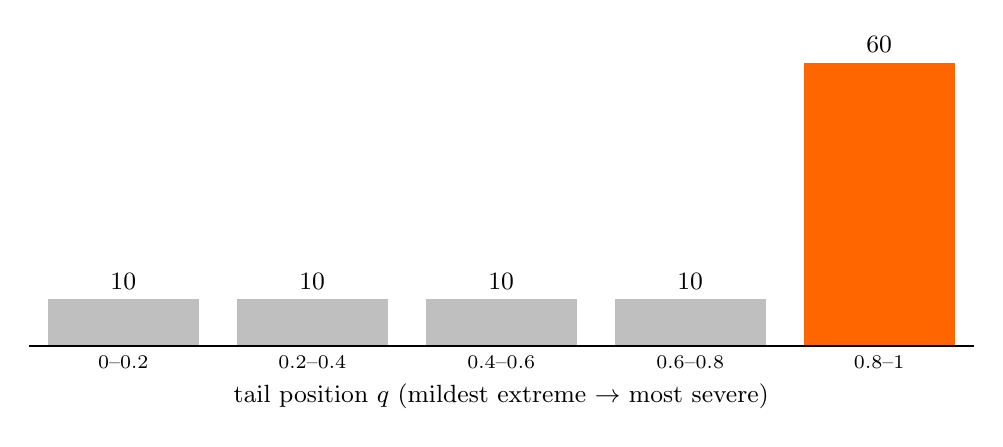
\begin{tikzpicture}[x=2.4cm,y=0.06cm]
\foreach \i/\v/\c in {0/10/black!25,1/10/black!25,2/10/black!25,3/10/black!25,4/60/orange!80!red}{
  \fill[\c] (\i+0.1,0) rectangle (\i+0.9,\v);
  \node[font=\small,anchor=south] at (\i+0.5,\v) {\v};}
\draw[thick] (0,0) -- (5,0);
\foreach \i/\l in {0/0--0.2,1/0.2--0.4,2/0.4--0.6,3/0.6--0.8,4/0.8--1}
  \node[font=\scriptsize,anchor=north] at (\i+0.5,0) {\l};
\node[font=\small,anchor=north] at (2.5,-6) {tail position $q$ (mildest extreme $\rightarrow$ most severe)};
\end{tikzpicture}
\caption{Of 100 added days, 10 fall in each of the four lower fifths (all from the ``anywhere'' half) and 60 in the top
fifth (10 + 50).}
\end{figure}

\begin{itemize}
  \item \textbf{Why not all 100 at the top?} Then the mild extremes would get no new examples and the model could get
        worse at them. Keeping half ``anywhere'' gives every part of the tail some new days.
  \item \textbf{Cap:} each $z$ is limited to the ceiling $\sigma/|\xi|$ and to 1.5 times the hottest real extreme of
        that season, so no added day is hotter than possible.
  \item \textbf{Plain (no EVT):} the comparison version simply uses severities as they occur in the real extremes.
\end{itemize}

\section{What EVT did not do in this project}
No block maxima, no GEV distribution, no return levels (``1-in-100-year heat''), and EVT was not built into the
training of the generators. It was used to \emph{rank} severity, to \emph{choose} the severities of added days, and to
\emph{cap} them.

\begin{sayit}
``Extreme value theory models only the tail. Above a high threshold, how far days go past it follows a generalised
Pareto distribution. I fitted one per season: the shape is negative, so heat has a ceiling. I then used it to put 60\%
of the added days in the rarest 20\% of the tail, and never above the ceiling.''
\end{sayit}

% =========================================================================
\chapter{Generative models}
\label{ch:gen}
% =========================================================================

\section{Neural network basics (just enough)}
A \textbf{neuron} multiplies each input $x_i$ by a weight $w_i$, adds them and a bias $b$, and passes the sum through
an \textbf{activation function} $f$ such as ReLU ($\max(0,z)$) or SiLU (a smooth version):
$\hat y=f(w_1x_1+\dots+w_nx_n+b)$. A \textbf{layer} is many neurons side by side; a \textbf{network} is layers in a row
(``$128\to128$'' means two layers of 128 neurons).

\begin{figure}[H]
\centering
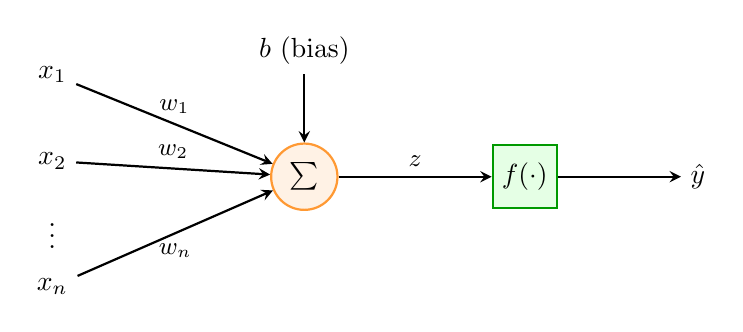
\begin{tikzpicture}[
  neuron/.style={circle,draw=blue!80,fill=blue!10,thick,minimum size=8mm},
  sum/.style={circle,draw=orange!80,fill=orange!10,thick,minimum size=8mm},
  act/.style={rectangle,draw=green!60!black,fill=green!10,thick,minimum size=8mm},
  arrow/.style={->,>=stealth,thick}]
\node (x1) at (0,1.6) {$x_1$}; \node (x2) at (0,0.5) {$x_2$}; \node at (0,-0.35) {$\vdots$}; \node (xn) at (0,-1.1) {$x_n$};
\node[sum] (s) at (3.2,0.3) {$\sum$}; \node[act] (f) at (6,0.3) {$f(\cdot)$}; \node (y) at (8.2,0.3) {$\hat y$};
\draw[arrow] (x1) -- node[above,font=\small]{$w_1$} (s); \draw[arrow] (x2) -- node[above,font=\small]{$w_2$} (s);
\draw[arrow] (xn) -- node[below,font=\small]{$w_n$} (s);
\node (b) at (3.2,1.9) {$b$ (bias)}; \draw[arrow] (b) -- (s);
\draw[arrow] (s) -- node[above,font=\small]{$z$} (f); \draw[arrow] (f) -- (y);
\end{tikzpicture}
\caption{One artificial neuron.}
\end{figure}

\textbf{Training} repeats three steps: (1) \emph{forward pass}: compute outputs and a \textbf{loss} (how wrong they
are); (2) \emph{backpropagation}: compute how the loss changes with every weight (the gradient); (3) \emph{update}: move
each weight a small step against its gradient (gradient descent; \textbf{Adam} and \textbf{AdamW} are popular versions
that adapt the step size). A \textbf{batch} is the number of rows used for one update; an \textbf{epoch} is one pass
over all training rows; the \textbf{learning rate} is the step size.

\section{What a generative model is}
A classifier learns to \emph{answer} (is this day extreme?). A \textbf{generative model} learns the \emph{shape of the
data} so it can \emph{produce new, realistic examples}. Here each generator learns from the 29{,}604 real extreme rows of
the training years and then produces new extreme rows: 49 numbers (the predictor groups A--D) plus the season. The 8
gap-to-threshold numbers (group E) are always recomputed afterwards. All three generators are trained from scratch.

\section{TVAE: a variational autoencoder}
\begin{figure}[H]
\centering
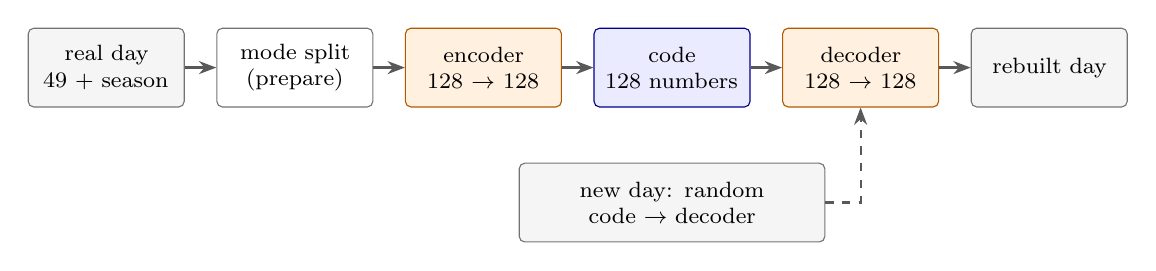
\begin{tikzpicture}[node distance=4mm]
\node[bdat,text width=1.7cm] (x) {real day\\49 + season};
\node[bx,text width=1.7cm,right=of x] (t) {mode split\\(prepare)};
\node[orange box,text width=1.7cm,right=of t] (e) {encoder\\$128\to128$};
\node[blue box,text width=1.7cm,right=of e] (h) {code\\128 numbers};
\node[orange box,text width=1.7cm,right=of h] (d) {decoder\\$128\to128$};
\node[bdat,text width=1.7cm,right=of d] (y) {rebuilt day};
\foreach \a/\b in {x/t,t/e,e/h,h/d,d/y} \draw[ar] (\a) -- (\b);
\node[bdat,text width=3.6cm,below=7mm of h] (n) {new day: random code $\rightarrow$ decoder};
\draw[ar,dashed] (n.east) -| (d.south);
\end{tikzpicture}
\caption{TVAE (Xu et al., NeurIPS 2019).}
\end{figure}
\begin{itemize}
  \item \textbf{Autoencoder:} the \emph{encoder} squeezes a day into a short \textbf{code} (also called the latent
        vector), the \emph{decoder} rebuilds the day from it. Learning to rebuild forces the code to capture what
        matters.
  \item \textbf{Variational:} the code is drawn from a bell curve with a learned mean $\mu$ and spread $\sigma$
        ($\mathbf h=\mu+\sigma\epsilon$, the \emph{reparameterisation trick}), and a \textbf{KL term} in the loss keeps
        all codes close to a standard bell curve. Then \emph{any} random code from that bell curve decodes to a
        sensible day: that is how new days are made.
  \item \textbf{Loss (ELBO):} rebuild error + KL term.
  \item \textbf{Tabular (``T''):} each number column is first split into its typical ranges (\emph{modes}) using a
        Gaussian mixture, so skewed columns such as rain are handled well.
  \item \textbf{Weakness:} rebuilding rewards typical rows, so it tends to average: its extremes are mostly mild. 75\%
        of its raw rows broke a physical rule before clean-up.
  \item \textbf{Settings:} code of 128, encoder and decoder of two layers of 128 (library defaults), 300 epochs,
        batch 500.
\end{itemize}

\section{CTGAN: a conditional generative adversarial network}
\begin{figure}[H]
\centering
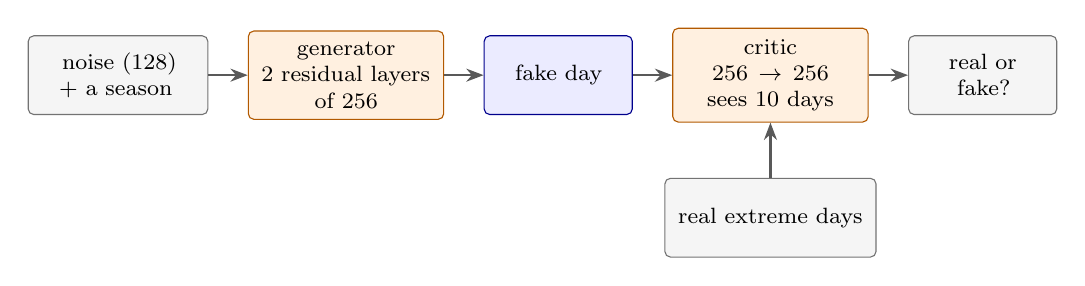
\begin{tikzpicture}[node distance=5mm]
\node[bdat,text width=2.0cm] (z) {noise (128)\\+ a season};
\node[orange box,text width=2.2cm,right=of z] (g) {generator\\2 residual layers\\of 256};
\node[blue box,text width=1.6cm,right=of g] (f) {fake day};
\node[orange box,text width=2.2cm,right=of f] (c) {critic\\$256\to256$\\sees 10 days};
\node[bdat,text width=1.6cm,right=of c] (s) {real or\\fake?};
\node[bdat,text width=2.4cm,below=7mm of c] (r) {real extreme days};
\foreach \a/\b in {z/g,g/f,f/c,c/s} \draw[ar] (\a) -- (\b);
\draw[ar] (r) -- (c);
\end{tikzpicture}
\caption{CTGAN (Xu et al., NeurIPS 2019).}
\end{figure}
\begin{itemize}
  \item \textbf{Two networks that compete:} the \emph{generator} turns random noise into a fake day; the \emph{critic}
        (discriminator) tries to tell fake days from real ones. Each improves against the other until fake days look
        real. Like a forger and a detective.
  \item \textbf{Conditional:} the generator is also given a season, and must produce a day of that season.
        \emph{Training-by-sampling} shows rare seasons often enough that they are learned.
  \item \textbf{WGAN-GP loss:} the critic gives a realness score rather than a yes/no, and a \emph{gradient penalty}
        keeps it smooth. This makes training more stable than the original GAN.
  \item \textbf{Packing (pac 10):} the critic judges 10 days together, so the generator cannot fool it by repeating one
        good day (\emph{mode collapse}).
  \item \textbf{Weakness:} it learns to fool the critic, not physics: 69\% of raw rows broke a rule. Strength: it
        reached the hot tail best on its own.
  \item \textbf{Settings:} noise of 128, generator and critic of two layers of 256 (library defaults), 300 epochs,
        batch 500, learning rate $2\times10^{-4}$.
\end{itemize}

\section{Conditional diffusion model (DDPM)}
\begin{figure}[H]
\centering
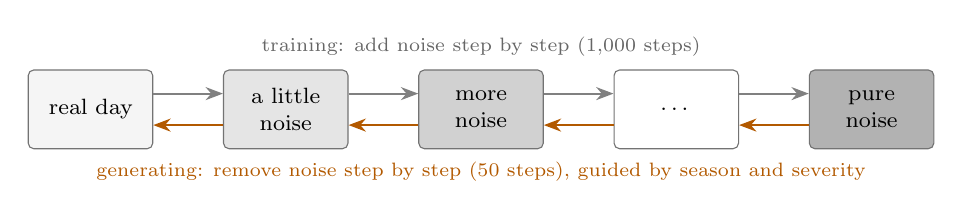
\begin{tikzpicture}[x=1.55cm]
\foreach \i/\l/\c in {0/real day/black!4,1/a little noise/black!10,2/more noise/black!18,3/\dots/white,4/pure noise/black!30}
  \node[bx,fill=\c,text width=1.3cm] (n\i) at (\i*1.6,0) {\l};
\foreach \i in {0,...,3} { \pgfmathtruncatemacro{\j}{\i+1}
  \draw[ar,black!50] ([yshift=2mm]n\i.east) -- ([yshift=2mm]n\j.west);
  \draw[ar,orange!70!black] ([yshift=-2mm]n\j.west) -- ([yshift=-2mm]n\i.east); }
\node[font=\scriptsize,black!60,anchor=south] at (3.2,0.55) {training: add noise step by step (1,000 steps)};
\node[font=\scriptsize,orange!70!black,anchor=north] at (3.2,-0.55) {generating: remove noise step by step (50 steps), guided by season and severity};
\end{tikzpicture}
\caption{The idea of diffusion (Ho et al., NeurIPS 2020).}
\end{figure}
\begin{itemize}
  \item \textbf{Forward process (training):} take a real day and add a little random noise, again and again, over
        1{,}000 steps, until nothing is left but noise. The amount added at each step follows a \emph{cosine
        schedule}.
  \item \textbf{What the network learns:} given a noisy day, how noisy it is (the step $t$), and the condition (season
        and severity $z$), guess the noise that was added. Loss = squared error of that guess.
  \item \textbf{Reverse process (generating):} start from pure noise and remove the guessed noise step by step. Using
        the \textbf{DDIM} shortcut, 50 steps are enough instead of 1{,}000.
  \item \textbf{Classifier-free guidance:} in training the condition is hidden 10\% of the time, so the same network
        can guess the noise with and without it. When generating, the two guesses are combined,
        $\tilde\epsilon=(1+w)\,\epsilon(\text{with condition})-w\,\epsilon(\text{without})$, with $w=2$: this pushes
        the day towards the requested season and severity.
  \item \textbf{Network:} the noisy day, the step and the condition are each turned into 512 numbers and added; four
        \emph{residual blocks} (each: normalise, widen to 1{,}024, SiLU, back to 512, and add its input back) predict
        the noise. About 4.85 million weights. Inputs are first mapped to a bell curve (quantile transform).
  \item \textbf{Training:} AdamW, learning rate $10^{-3}$, 15{,}000 steps of 1{,}024 rows, and an averaged copy of the
        weights (EMA 0.999) used for generating.
  \item \textbf{Strengths:} can be \emph{asked} for an exact season and severity (the only one of the three); almost no
        raw rows broke physics; its days were the closest to real ones.
\end{itemize}

\section{From generator to training data}
\begin{figure}[H]
\centering
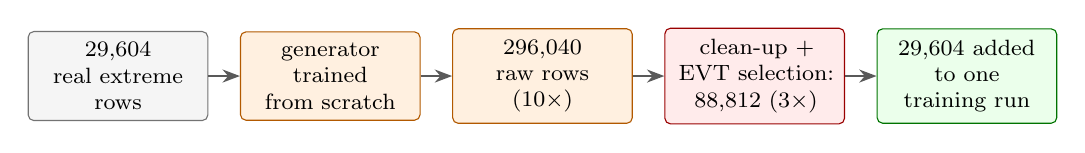
\begin{tikzpicture}[node distance=4mm]
\node[bdat,text width=2.0cm] (a) {29{,}604\\real extreme\\rows};
\node[orange box,text width=2.0cm,right=of a] (b) {generator\\trained\\from scratch};
\node[orange box,text width=2.0cm,right=of b] (c) {296{,}040\\raw rows\\($10\times$)};
\node[red box,text width=2.0cm,right=of c] (d) {clean-up +\\EVT selection:\\88{,}812 ($3\times$)};
\node[green box,text width=2.0cm,right=of d] (e) {29{,}604 added\\to one\\training run};
\foreach \u/\v in {a/b,b/c,c/d,d/e} \draw[ar] (\u) -- (\v);
\end{tikzpicture}
\caption{Counts for TVAE and CTGAN. The diffusion model is asked directly for the EVT severities.}
\end{figure}
\begin{itemize}
  \item \textbf{Consistency clean-up} (the code calls it ``physics''; say ``consistency and range clean-up''):
        each generated row is moved to the nearest real cell (taking its real height and slope); the three daily
        temperatures are \emph{sorted} so that minimum $\le$ mean $\le$ maximum; dewpoint is capped at the mean
        temperature; humidity is cut to 0--100\%; rain and sunshine are cut at 0; soil water is cut to 0--0.8; counts
        are cut to range and rounded; the 8 gap columns are recomputed from that cell's threshold. It removes
        impossible values; it does \emph{not} make a day realistic (see the box below).
  \item \textbf{Judge model (TVAE and CTGAN only):} these two cannot be asked for a severity, so a separate LightGBM
        model, trained on real extremes, estimates the severity $z$ of each generated row; rows are then picked so that
        their tail positions match the EVT target (60\% in the top fifth) and their seasons match the real shares.
  \item \textbf{Placement:} the season follows the share of real extremes per season; the location is generated with
        the day and snapped to a real cell; so new days appear where extremes really occur.
\end{itemize}


\begin{keyidea}[What the clean-up does not do (say it before they ask)]
\begin{itemize}
  \item Humidity is not recomputed after the dewpoint is capped, so humidity, temperature and dewpoint can disagree.
  \item Temperature is not checked against the height of the cell the row is snapped to (a 40\,$^\circ$C row can land
        on a 4{,}000\,m cell; its gap columns then become very large).
  \item Anomaly and 7--30-day history columns are not recomputed from the daily values.
\end{itemize}
Real data break none of the rules (about 0\%); raw TVAE rows broke at least one in 75\% of cases, CTGAN in 69\%, the
diffusion model in about 0\%.
\end{keyidea}

\begin{keyidea}[Why 0.8 for soil moisture?]
\textbf{What the number is.} Soil moisture here (\texttt{swvl1}) is \emph{volumetric}: the fraction of the top 7\,cm
of soil that is water, in m$^3$\,m$^{-3}$. It can never be larger than the share of the soil that is empty space
(its \emph{saturation} or porosity): once every pore is full, no more water fits.

\textbf{What ERA5-Land allows.} ERA5-Land's land model (H-TESSEL) gives each soil texture a saturation value taken
from the European HYPRES soil table: about 0.40 for coarse (sandy) soil and at most 0.766 for organic soil. So the
model itself can never produce more than about 0.77.

\textbf{What our data show.} Over all 529 cells and all days 1981--2025, \texttt{swvl1} ranged from 0.012 to
\textbf{0.751} (median 0.304), from the Step 1 check.

\textbf{So why 0.8?} It is a round upper bound chosen by us, just above both the model's maximum (0.766) and the
largest real value (0.751). It therefore never cuts a value that real data could contain; it only removes generated
values that are impossible (above 0.8, or below 0). It is a sanity limit, not a physical constant.

\textbf{Honest weakness.} A stricter choice would use each cell's own soil saturation (or its highest value in
1981--2010): a value of 0.78 is impossible for a mineral soil but still passes 0.8.
\end{keyidea}

\begin{sayit}
``TVAE compresses a day into a code and rebuilds it; new codes give new days. CTGAN is a generator and a critic that
compete. The diffusion model learns to remove noise step by step and can be asked for a season and a severity. Each
learns from the 29,604 real extremes, and every generated day is cut to valid ranges, made internally consistent and placed on a real cell.''
\end{sayit}

% =========================================================================
\chapter{The classifier: LightGBM}
\label{ch:clf}
% =========================================================================

\section{Decision trees}
A \textbf{decision tree} asks a chain of yes/no questions about the predictors (``is the gap to the threshold smaller
than 1\,$^\circ$C?'', ``has it been dry for 30 days?'') and ends in a \textbf{leaf} that holds an answer. One tree is
simple but weak.

\begin{figure}[H]
\centering
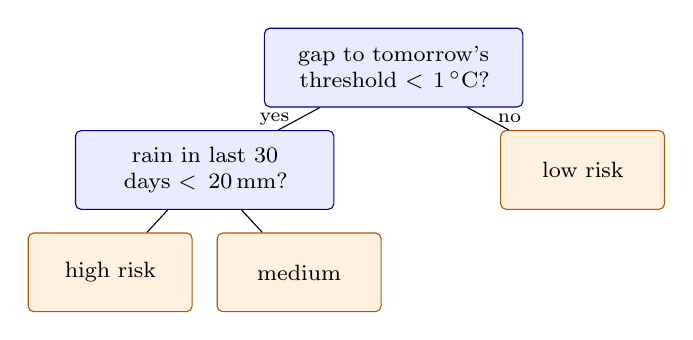
\begin{tikzpicture}[level distance=13mm,
  level 1/.style={sibling distance=48mm},level 2/.style={sibling distance=24mm},
  q/.style={bx,fill=blue!8,draw=blue!55!black,text width=3.0cm},
  lf/.style={bx,fill=orange!12,draw=orange!70!black,text width=1.8cm}]
\node[q] {gap to tomorrow's threshold $<1\,^\circ$C?}
  child {node[q] {rain in last 30 days $<20$\,mm?}
     child {node[lf] {high risk}} child {node[lf] {medium}}
     edge from parent node[left,font=\scriptsize] {yes}}
  child {node[lf] {low risk} edge from parent node[right,font=\scriptsize] {no}};
\end{tikzpicture}
\caption{A toy decision tree (illustrative questions, not the learned ones).}
\end{figure}

\section{Gradient boosting and LightGBM}
\textbf{Gradient boosting} builds many small trees one after another; each new tree corrects the mistakes the previous
trees still make. The prediction is the sum of all trees, turned into a probability. \textbf{LightGBM} (Ke et al.,
NeurIPS 2017) is a fast implementation of this.

\begin{center}
\footnotesize
\begin{tabular}{p{4.5cm}p{9.2cm}}
\toprule
\textbf{Setting} & \textbf{Meaning}\\
\midrule
learning rate 0.05 & each new tree adds only 5\% of its correction, so learning is careful\\
31 leaves per tree & how detailed one tree can be\\
at least 200 rows per leaf & stops trees from memorising tiny groups\\
80\% of rows and of columns per tree & each tree sees a random part of the data, which reduces overfitting\\
up to 1{,}000 trees, early stopping 60 & training stops when 60 new trees in a row do not improve the validation score\\
monotone constraint & a smaller gap to the threshold (predictors \texttt{dist\_l0} and \texttt{dist\_std\_l0}) can never lower the
  predicted risk: a physics rule built into the model\\
5 seeds & trained 5 times with different random choices; results are the mean, or the 5 predictions averaged\\
\bottomrule
\end{tabular}
\end{center}

\section{Why LightGBM and not a neural network}
\begin{itemize}
  \item On table data, tree models are usually stronger than neural networks (Grinsztajn et al., NeurIPS 2022).
  \item It trains on 2.9 million rows on a normal CPU, without a GPU.
  \item It allows the monotone (physics) constraint, and shows which predictors matter most.
  \item A neural network (multilayer perceptron, three layers of 256) was tried in an early run: about the same score
        on real data (0.597 vs 0.594), but slower and needing a GPU.
  \item Keeping \textbf{one fixed classifier} means any difference in the results comes from the added data, not from
        the model.
\end{itemize}

\section{From probability to warning}
LightGBM outputs a probability for each row. A \textbf{warning cut-off} turns it into yes/no: warn if the probability
is above the cut-off. The cut-off is chosen on the validation years as the one with the best F1 score
(Chapter~\ref{ch:metrics}), never on the test years.

\begin{sayit}
``LightGBM builds many small decision trees, each correcting the previous ones. It is strong on tables, fast on a CPU,
and lets me add a physics rule: closer to the threshold never means lower risk. Keeping it fixed means differences in
results come from the data I add.''
\end{sayit}

% =========================================================================
\chapter{How the warnings are scored}
\label{ch:metrics}
% =========================================================================

\section{The confusion matrix}
Every test row ends in one of four boxes:
\begin{center}
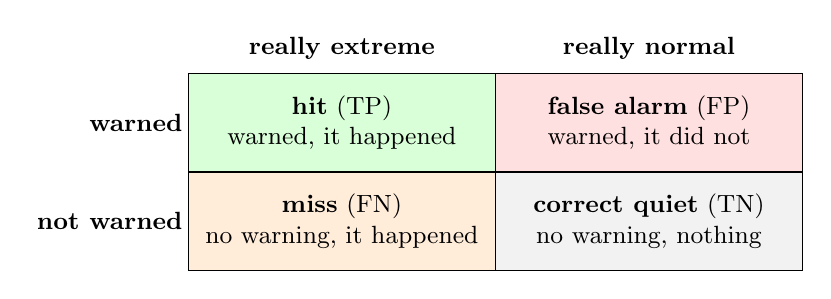
\begin{tikzpicture}[cell/.style={draw,minimum width=3.9cm,minimum height=1.25cm,align=center,font=\small}]
\node[cell,fill=green!15] at (0,0) {\textbf{hit} (TP)\\warned, it happened};
\node[cell,fill=red!12] at (3.9,0) {\textbf{false alarm} (FP)\\warned, it did not};
\node[cell,fill=orange!15] at (0,-1.25) {\textbf{miss} (FN)\\no warning, it happened};
\node[cell,fill=black!5] at (3.9,-1.25) {\textbf{correct quiet} (TN)\\no warning, nothing};
\node[font=\small\bfseries] at (0,0.95) {really extreme};
\node[font=\small\bfseries] at (3.9,0.95) {really normal};
\node[font=\small\bfseries,anchor=east] at (-1.9,0) {warned};
\node[font=\small\bfseries,anchor=east] at (-1.9,-1.25) {not warned};
\end{tikzpicture}
\end{center}

\section{The measures}
\begin{center}
\footnotesize
\begin{tabular}{p{3.0cm}p{3.6cm}p{7.2cm}}
\toprule
\textbf{Measure} & \textbf{Formula} & \textbf{Plain meaning}\\
\midrule
Precision & TP/(TP+FP) & of the warnings issued, the share that were right\\
Recall (hit rate) & TP/(TP+FN) & of the extreme days, the share that were warned\\
F1 & $2PR/(P+R)$ & one number balancing precision $P$ and recall $R$\\
CSI (threat score) & TP/(TP+FP+FN) & used in weather services; ignores the many correct quiet days\\
False-alarm rate & FP/(FP+TN) & of the normal days, the share wrongly warned\\
Accuracy & (TP+TN)/all & misleading here: saying ``never extreme'' scores 98.1\% on the test years\\
\bottomrule
\end{tabular}
\end{center}

\begin{keyidea}[Why not accuracy]
Only 1.94\% of test rows are extreme. A model that never warns is right 98.1\% of the time and useless. That is why
the project uses PR-AUC.
\end{keyidea}

\section{PR curve and PR-AUC}
Moving the warning cut-off from high to low gives a different (precision, recall) pair each time. Plotting them gives
the \textbf{precision--recall curve}; the area under it is \textbf{PR-AUC} (computed as \emph{average precision}, AP).
It is 1 for a perfect model, and equal to the share of extremes (about 0.02 on the test years) for random guessing.

\begin{example}[Five days by hand]
The model gives: A 0.9 (extreme), B 0.7 (normal), C 0.6 (extreme), D 0.3 (normal), E 0.1 (normal).
Go down the list. At A: precision $1/1=1$ (first extreme found). At C: precision $2/3$ (two extremes among three
warnings). AP = mean of the precision at each extreme $=(1+2/3)/2=0.83$. If C had been ranked above B, AP would be 1.
\end{example}

\begin{figure}[H]
\centering
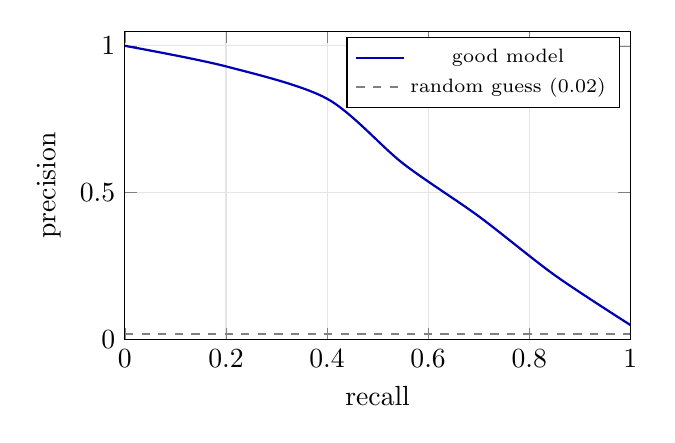
\begin{tikzpicture}
\begin{axis}[width=8cm,height=5.5cm,xlabel={recall},ylabel={precision},xmin=0,xmax=1,ymin=0,ymax=1.05,
  legend style={font=\scriptsize,at={(0.98,0.98)},anchor=north east},grid=major,grid style={black!10}]
\addplot[blue!70!black,thick,smooth] coordinates {(0,1)(0.2,0.93)(0.4,0.82)(0.55,0.6)(0.7,0.42)(0.85,0.22)(1,0.05)};
\addlegendentry{good model}
\addplot[black!50,dashed,thick] coordinates {(0,0.02)(1,0.02)};
\addlegendentry{random guess (0.02)}
\end{axis}
\end{tikzpicture}
\caption{Illustrative PR curve. The area under the blue line is the PR-AUC.}
\end{figure}

\textbf{Why PR and not ROC:} the ROC curve uses the false-alarm rate, whose denominator is the huge number of normal
days, so even many false alarms look small and ROC-AUC looks excellent for weak models. PR-AUC focuses on the rare
class, which is the one that matters.

\section{The three test subsets}
\begin{itemize}
  \item \textbf{All days:} every test row (1,932,437 rows, 37,450 extreme).
  \item \textbf{Severe:} all normal rows plus only the 10\% most severe extreme rows (largest $z$). It asks: can the
        model catch the worst heat? This is the main score of the project.
  \item \textbf{Onset:} only rows where today's maximum is still below tomorrow's threshold. The model cannot simply
        say ``hot today, so hot tomorrow''; it must predict the \emph{start} of an extreme.
\end{itemize}

\section{Per-seed mean vs combined model}
Each setting is trained with 5 seeds. The \textbf{per-seed mean} averages the 5 scores (it shows how consistent the
gain is, and ``runs better'' counts how many of the 5 seeds beat real-only). The \textbf{combined (ensemble)} score
averages the 5 predicted probabilities first and scores that; it is a little higher, and is what you would use in
practice.

\begin{sayit}
``Accuracy is meaningless when 98\% of days are normal, so I use PR-AUC, the area under the precision--recall curve.
Random guessing scores 0.02. I report it on all days, on the most severe 10\% of extremes, and on onset days.''
\end{sayit}

% =========================================================================
\chapter{Results and what they mean}
\label{ch:results}
% =========================================================================

\section{Main result: severe days}
\begin{center}
\begin{tabular}{lccc}
\toprule
\textbf{Training data} & \textbf{Severe PR-AUC} & \textbf{Change} & \textbf{All days}\\
\midrule
Real data only & 0.441 & -- & 0.599\\
Real + DDPM & 0.579 & +31\% & 0.609--0.611\\
Real + TVAE & 0.601 & +36\% & 0.609--0.611\\
Real + CTGAN & 0.601 & +36\% & 0.609--0.611\\
\bottomrule
\end{tabular}
\end{center}
Combined (5-seed ensemble) scores. Adding EVT-guided synthetic extremes raises the severe score by about a third, while
the all-days score also rises slightly, so nothing is lost on ordinary extremes.

\begin{figure}[H]
\centering
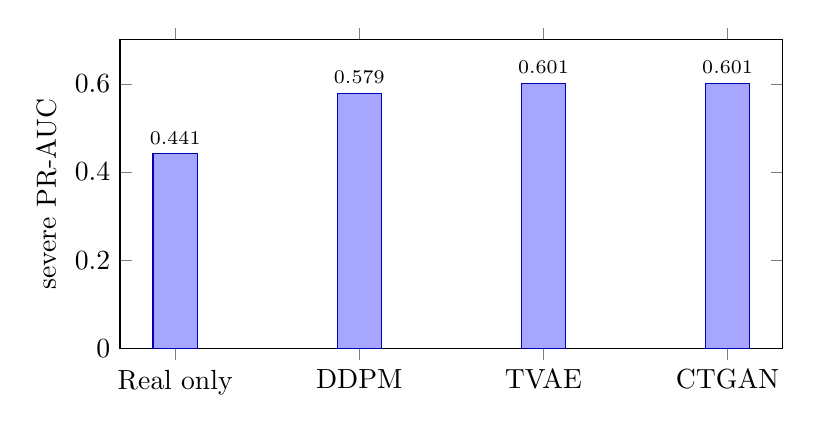
\begin{tikzpicture}
\begin{axis}[ybar,width=10cm,height=5.5cm,bar width=16pt,ymin=0,ymax=0.7,ylabel={severe PR-AUC},
  symbolic x coords={Real only,DDPM,TVAE,CTGAN},xtick=data,nodes near coords,
  nodes near coords style={font=\scriptsize},every node near coord/.append style={/pgf/number format/fixed,/pgf/number format/precision=3}]
\addplot[fill=blue!35,draw=blue!70!black] coordinates {(Real only,0.441)(DDPM,0.579)(TVAE,0.601)(CTGAN,0.601)};
\end{axis}
\end{tikzpicture}
\caption{Severe-day PR-AUC, combined model.}
\end{figure}

\section{Does the EVT tail matter? (per-seed means, severe days)}
\begin{center}
\begin{tabular}{lcccc}
\toprule
\textbf{Generator} & \textbf{Plain} & \textbf{EVT tail} & \textbf{Gain} & \textbf{Runs better}\\
\midrule
DDPM & 0.482 & 0.549 & +13.8\% & 5/5\\
TVAE & 0.514 & 0.583 & +13.6\% & 5/5\\
CTGAN & 0.554 & 0.581 & +4.9\% & 3/5\\
\bottomrule
\end{tabular}
\end{center}
``Plain'' = the same number of synthetic days, but chosen without EVT (their severities follow the generator).
Real data only scores 0.411 on this per-seed basis. EVT helps all three; it helps CTGAN least because CTGAN already
reaches the hot tail by itself.

\section{Checks that support the method}
\begin{itemize}
  \item \textbf{GPD as-is} (sample tail positions straight from the fitted GPD, no extra weight on the top fifth):
        0.462, better in only 1 of 5 runs. The \emph{tail focus} is what helps.
  \item \textbf{Random copies control:} adding copies of random real extremes gives 0.464; copying real extremes
        chosen by the EVT tail rule gives 0.521 (5/5, all-days 0.608). So the tail rule helps even without a
        generator, and new generated days help more.
  \item \textbf{How many to add:} 1 synthetic per real extreme gave onset 0.222; 8.7 per extreme gave 0.197. More is not
        better: too many synthetic days drown the real ones.
\end{itemize}

\section{In practice (CTGAN, combined model, chosen cut-off)}
Precision 0.600, recall 0.550, false-alarm rate 0.7\%: of every 10 warnings, 6 are right; a little over half of the
extreme days are warned; fewer than 1 in 100 normal days gets a false warning.

\section{Limitations (say these before they are asked)}
\begin{itemize}
  \item One region and one dataset (ERA5-Land, a reanalysis, not station readings; not bias-corrected).
  \item Thresholds come from 1981--2010; the test years are warmer (1.94\% extremes vs 1\%), so the task shifts.
  \item Synthetic days are judged only by whether they help the classifier, not checked by a meteorologist.
  \item GPD fitted by pooling cells within a season; it ignores differences between cells.
  \item Only next-day prediction; longer lead times were not tried.
\end{itemize}

\begin{sayit}
``With real data alone the severe score is 0.441. Adding EVT-guided synthetic extremes raises it to 0.58--0.60, about
a third better, without hurting the all-days score. The controls show the gain comes from focusing on the tail, not
just from adding more rows.''
\end{sayit}

% =========================================================================
\chapter{Likely questions and short answers}
\label{ch:questions}
% =========================================================================

\newcommand{\qa}[2]{\par\medskip\noindent\textbf{Q. #1}\par\noindent #2\par}

\qa{What is extreme value theory?}{The branch of statistics for the largest values. Its key result
(Pickands--Balkema--de Haan) says the excesses above a high threshold follow a generalised Pareto distribution
(GPD), whatever the original distribution.}

\qa{What does $\xi$ tell you?}{The shape of the tail. Negative (as here, about $-0.15$): the tail has an upper limit,
which is physical for temperature. Zero: exponential tail. Positive: heavy tail with no limit.}

\qa{Why not just oversample (SMOTE or copies)?}{Copies add no new information, and SMOTE only draws between existing
points, so neither reaches beyond the hottest day seen. The control shows random copies give 0.464 against 0.58--0.60
with EVT-guided generated days.}

\qa{How do you know the generated days are realistic?}{Every row is cleaned to obey physical rules and placed on a real
cell; the 8 gap columns are recomputed; and the test is done only on real days from 2016--2025, which the generators
never saw.}

\qa{Why the 99th percentile?}{It gives about 1\% extremes per cell and season, rare enough to be ``extreme'' but with
enough cases (29,604 in training) to learn from. It is computed separately per cell and season, so a hot day in Kinnaur
and in Una are judged on their own scales.}

\qa{Why 1981--2010 for thresholds?}{It is a standard 30-year WMO climate normal period, and it keeps the thresholds
fixed before the validation and test years.}

\qa{Why was the test set not split randomly?}{Days close in time are similar; a random split would leak information.
Validation and test are later, separate years.}

\qa{Is there leakage from tomorrow?}{No. All predictors use today and earlier; only the label looks at tomorrow.}

\qa{Why LightGBM?}{Best known model type for tables, fast on CPU, allows the physics (monotone) constraint. An MLP
scored the same on real data. One fixed classifier means differences come from the data.}

\qa{Why does CTGAN gain less from EVT?}{Without EVT it already produced many hot-tail days (plain score 0.554, the
highest), so there was less to fix.}

\qa{What is the 60\%?}{Tail positions are drawn half from the whole tail and half from its top fifth, so
$0.5\times0.2+0.5\times1=0.6$: 60\% of added days fall in the top 20\% of the tail.}

\qa{Why cap the severity?}{With $\xi<0$ the GPD has an end point $\sigma/|\xi|$; going past it is impossible. The cap
also stops anything above 1.5 times the hottest real excess.}

\qa{Why 529 cells?}{The ERA5-Land grid (0.1$^\circ$) over the box around Himachal Pradesh has $31\times37=1{,}147$
cells; 529 have their centre inside the state boundary.}

\qa{Why cap soil moisture at 0.8?}{Soil moisture is the fraction of the soil that is water and cannot exceed the
soil's saturation. In ERA5-Land's land model the largest saturation is 0.766 (organic soil), and our data never went
above 0.751. So 0.8 is a round limit just above anything real: it removes only impossible generated values and never
cuts a realistic one. It is our choice, not a constant; a per-cell limit would be stricter.}

\qa{Is the physics clean-up real physics?}{No, it is a consistency and range clean-up: rows are placed on a real
cell, values are cut to valid ranges, temperatures are ordered and the gap columns recomputed. It removes impossible
values but does not check a day against a weather model; humidity and the history columns are not recomputed.}

\qa{What would you do next?}{Longer lead times; let the GPD vary by cell or with elevation; check synthetic days with a
meteorologist; try the method in another region.}

% =========================================================================
\chapter*{Glossary}
\addcontentsline{toc}{chapter}{Glossary}
% =========================================================================
\begin{description}[style=nextline,leftmargin=0pt,itemsep=3pt,font=\bfseries]
\footnotesize
\item[Anomaly] Today's value minus the normal value for that calendar day (1981--2010 mean over $\pm7$ days).
\item[Average precision (AP)] The way PR-AUC is computed: mean precision at each correctly found extreme.
\item[Batch / epoch] Rows used per training update / one full pass over the training data.
\item[Bootstrap] Refitting many times on resampled data (here, whole days, 100 times) to get a range of uncertainty.
\item[Cell] One 0.1$^\circ$ ERA5-Land grid square, about $9.4\times11.1$\,km. 529 cover Himachal Pradesh.
\item[Class imbalance] One class (normal days) far outnumbers the other (extreme days, about 1--2\%).
\item[Classifier-free guidance] Mixing the diffusion model's guesses with and without the condition to follow it more strongly ($w=2$).
\item[Climate normal] A 30-year reference period; here 1981--2010.
\item[Conditional] A generator that can be told what to produce (season; for DDPM also severity).
\item[CTGAN] Conditional tabular GAN: generator and critic competing.
\item[DDIM] A faster way to run the diffusion reverse process (50 steps instead of 1,000).
\item[DDPM] Denoising diffusion probabilistic model: learns to remove noise step by step.
\item[DEM] Digital elevation model: a map of ground height (here SRTM).
\item[Early stopping] Stop adding trees when the validation score has not improved for 60 rounds.
\item[Ensemble] The average of the 5 seeds' predicted probabilities.
\item[ERA5-Land] ECMWF's land reanalysis: hourly/daily weather on a 0.1$^\circ$ grid since 1950.
\item[EVT] Extreme value theory: statistics of the largest values.
\item[Extreme day] A day whose maximum temperature is above that cell's 99th percentile for the season.
\item[F1] Balance of precision and recall; used to pick the warning cut-off on the validation years.
\item[GADM] Database of administrative boundaries; gives the state outline.
\item[GAN] Generative adversarial network: generator vs critic.
\item[GPD] Generalised Pareto distribution, the law of excesses over a high threshold; parameters $\xi$ (shape), $\sigma$ (scale).
\item[LightGBM] A fast gradient-boosted decision-tree library; the fixed classifier.
\item[Monotone constraint] A rule that the prediction can only rise as a predictor rises (here, closer to the threshold).
\item[MLE] Maximum likelihood estimation: choose parameters that make the observed data most likely.
\item[Onset] A day that becomes extreme tomorrow while today is still below tomorrow's threshold.
\item[Percentile] The value below which a given share of data lies (99th: 99\% below).
\item[PR-AUC] Area under the precision--recall curve; random = share of extremes.
\item[Precision / recall] Share of warnings that were right / share of extremes that were warned.
\item[Predictor (feature)] One input number of a row; there are 57.
\item[Reanalysis] Weather model + all observations combined to give a complete past record.
\item[Seed] The starting number for random choices; 5 seeds = 5 independent training runs.
\item[Severe subset] All normal days plus the 10\% most severe extremes.
\item[SMOTE] Oversampling by drawing new points between existing minority points.
\item[SRTM] Shuttle Radar Topography Mission; 30\,m elevation data.
\item[Standardised excess $z$] $(T_{\max}-u)/s$: how far above the threshold, in units of that cell's typical day-to-day spread.
\item[Tail position $q$] Where $z$ sits in the fitted GPD, from 0 (just above the threshold) to 1 (most extreme).
\item[Threshold $u$] The 99th percentile per cell and season; 2,116 in all.
\item[TVAE] Tabular variational autoencoder: encoder, code, decoder.
\item[Validation / test] Years for tuning (2011--15) / years for the final honest score (2016--25).
\item[$\xi$ (xi)] GPD shape: negative means a bounded tail.
\end{description}


\end{document}
